\chapter{Implementación} 
\epigraph{\textit{I believe that at the end of the century the use of words and general educated opinion will have altered so much that one will be able to speak of machines thinking without expecting to be contradicted.     
	}}{\textit{—  Alan Turing, Computing machinery and intelligence}}
	\vspace*{8cm}
	\begin{center}
		\centering
		\includegraphics[width=10.5cm]{example-image}
	\end{center}
	\thispagestyle{empty}
	\newpage
\vspace*{2cm}

\section{Desarrollo de logo}
Se presenta el logo de SISPREL.
\begin{figure}[!htb]
    \centering
    
\includegraphics[scale=0.25]{TT/img/sisprel.png}
    \caption{Logo de SISPREL}
    \label{graphic:SISPRELLogo}    
\end{figure}

\section{Estructura del proyecto}
Para tener un control del proyecto, se presenta a continuación la estructura general con la cual se ha trabajado para tener una buena organización del sistema y sea fácil de entender donde va cada módulo del sistema, mas adelante se ahondará mas en cada sección del sistema.

\begin{enumerate}
    \item Frontend: En esta carpeta se almacenarán los módulos y el proyecto del Frontend del sistema, será desarrollado con JavaScript con el Framework VueJS
    \item Backend: En esta carpeta se almacenará el entorno de Python con los paquetes y el sistema desarrollado.
    \item Scripts: En esa carpeta se encontrarán los Scripts necesarios para construir y levantar de manera local el contenedor o subirlo en algun servicio en la nube.
    \item Raíz: En la carpeta raíz o donde se encuentran las carpetas mencionadas anteriormente, se encuentran algunos archivos de configuración de los contenedores asi mismo un archivo .env donde se almacenan variables como puertos, contraseña, URLs y otras cosas para que los archivos de configuración de Docker los usen y al momento de modificar alguna variable solo se tenga que hacer en un solo archivo y de manera general.
\end{enumerate}

\begin{figure}[!htb]
    \centering
    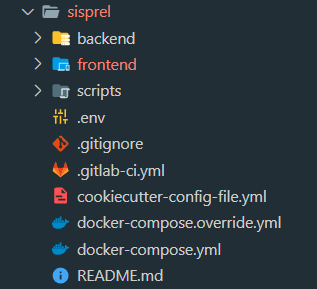
\includegraphics[scale=0.95]{TT/img/implementacion/carpetasGeneral.png}
    \caption{Estructura general de SISPREL}
    \label{graphic:carpetasGeneral}    
\end{figure}


\section{Configuración del entorno del sistema}
Para el desarrollo del sistema y poder trabajarlo en cualquier lugar sin tener que hacer instalaciones o configuraciones para cada sistema operativo, se optó por usar contenedores. Para ello, se eligió el software de Docker para llevar acabo este fin. 

El proyecto fue dividido en 4 contenedores, los cuales son:
\begin{enumerate}
    \item Proxy: Traefik 2.2
    \item DB: Postgres 12
    \item Backend: FastAPI
    \item Frontend: VueJS
\end{enumerate}

\subsection{Traefik}
Traefik es un enrutador/proxy inverso y un balanceador HTTP, TCP y UDP. Una herramienta que permite conectar distintas URL con el servicio que se requiera. Proporciona funcionalidades de intermediario que aumenta sus capacidades para realizar balanceo de carga o servir como gateway API. Además integra una Interfaz de usuario muy completa que nos da información sobre todo lo que ofrece. Para acceder a esta herramienta en el proyecto, de manera local se accede con la URL: localhost:8090.

\begin{figure}[!htb]
    \centering
    
\includegraphics[scale=0.1]{TT/img/implementacion/Traefik.logo.png}
    \caption{Logo de Traefik}
    \label{graphic:TraefikLogo}    
\end{figure}

Sus principales características son:
\begin{itemize}
    \item \textbf{Enrutado y balanceo de carga: }capa de enrutado flexible en la capa 4 y 7, soporta los protocolos HTTP, HTTP/2, TCP, UDP, Websockets, gRPC, despliegues blue-green y canary, fijación de sesión o session stickness y comprobaciones de salud.
    \item \textbf{Seguridad: }automatización de HTTP, soporte para Let’s Encrypt, certificados personalizados y autenticación.
    \item \textbf{Configuración dinámica: }a través de descubrimiento de servicios (Kubernetes, Docker Swarm, Red Hat OpenShift, Rancher, Amazon ECS, key-value stores) y funcionales de intermediario o middelware (circuit breakers, reintentos, buffering, compresión de la respuesta, cabeceras o limitación de peticiones).
    \item \textbf{Observabilidad: }posee un panel informativo de forma nativa, trazabilidad distribuida (Jaeger, Open Tracing, Zipkin) y métricas en tiempo real (Datadog, Grafana, InfluxDB, Prometheus, StatsD).
\end{itemize}

\begin{figure}[!htb]
    \centering
    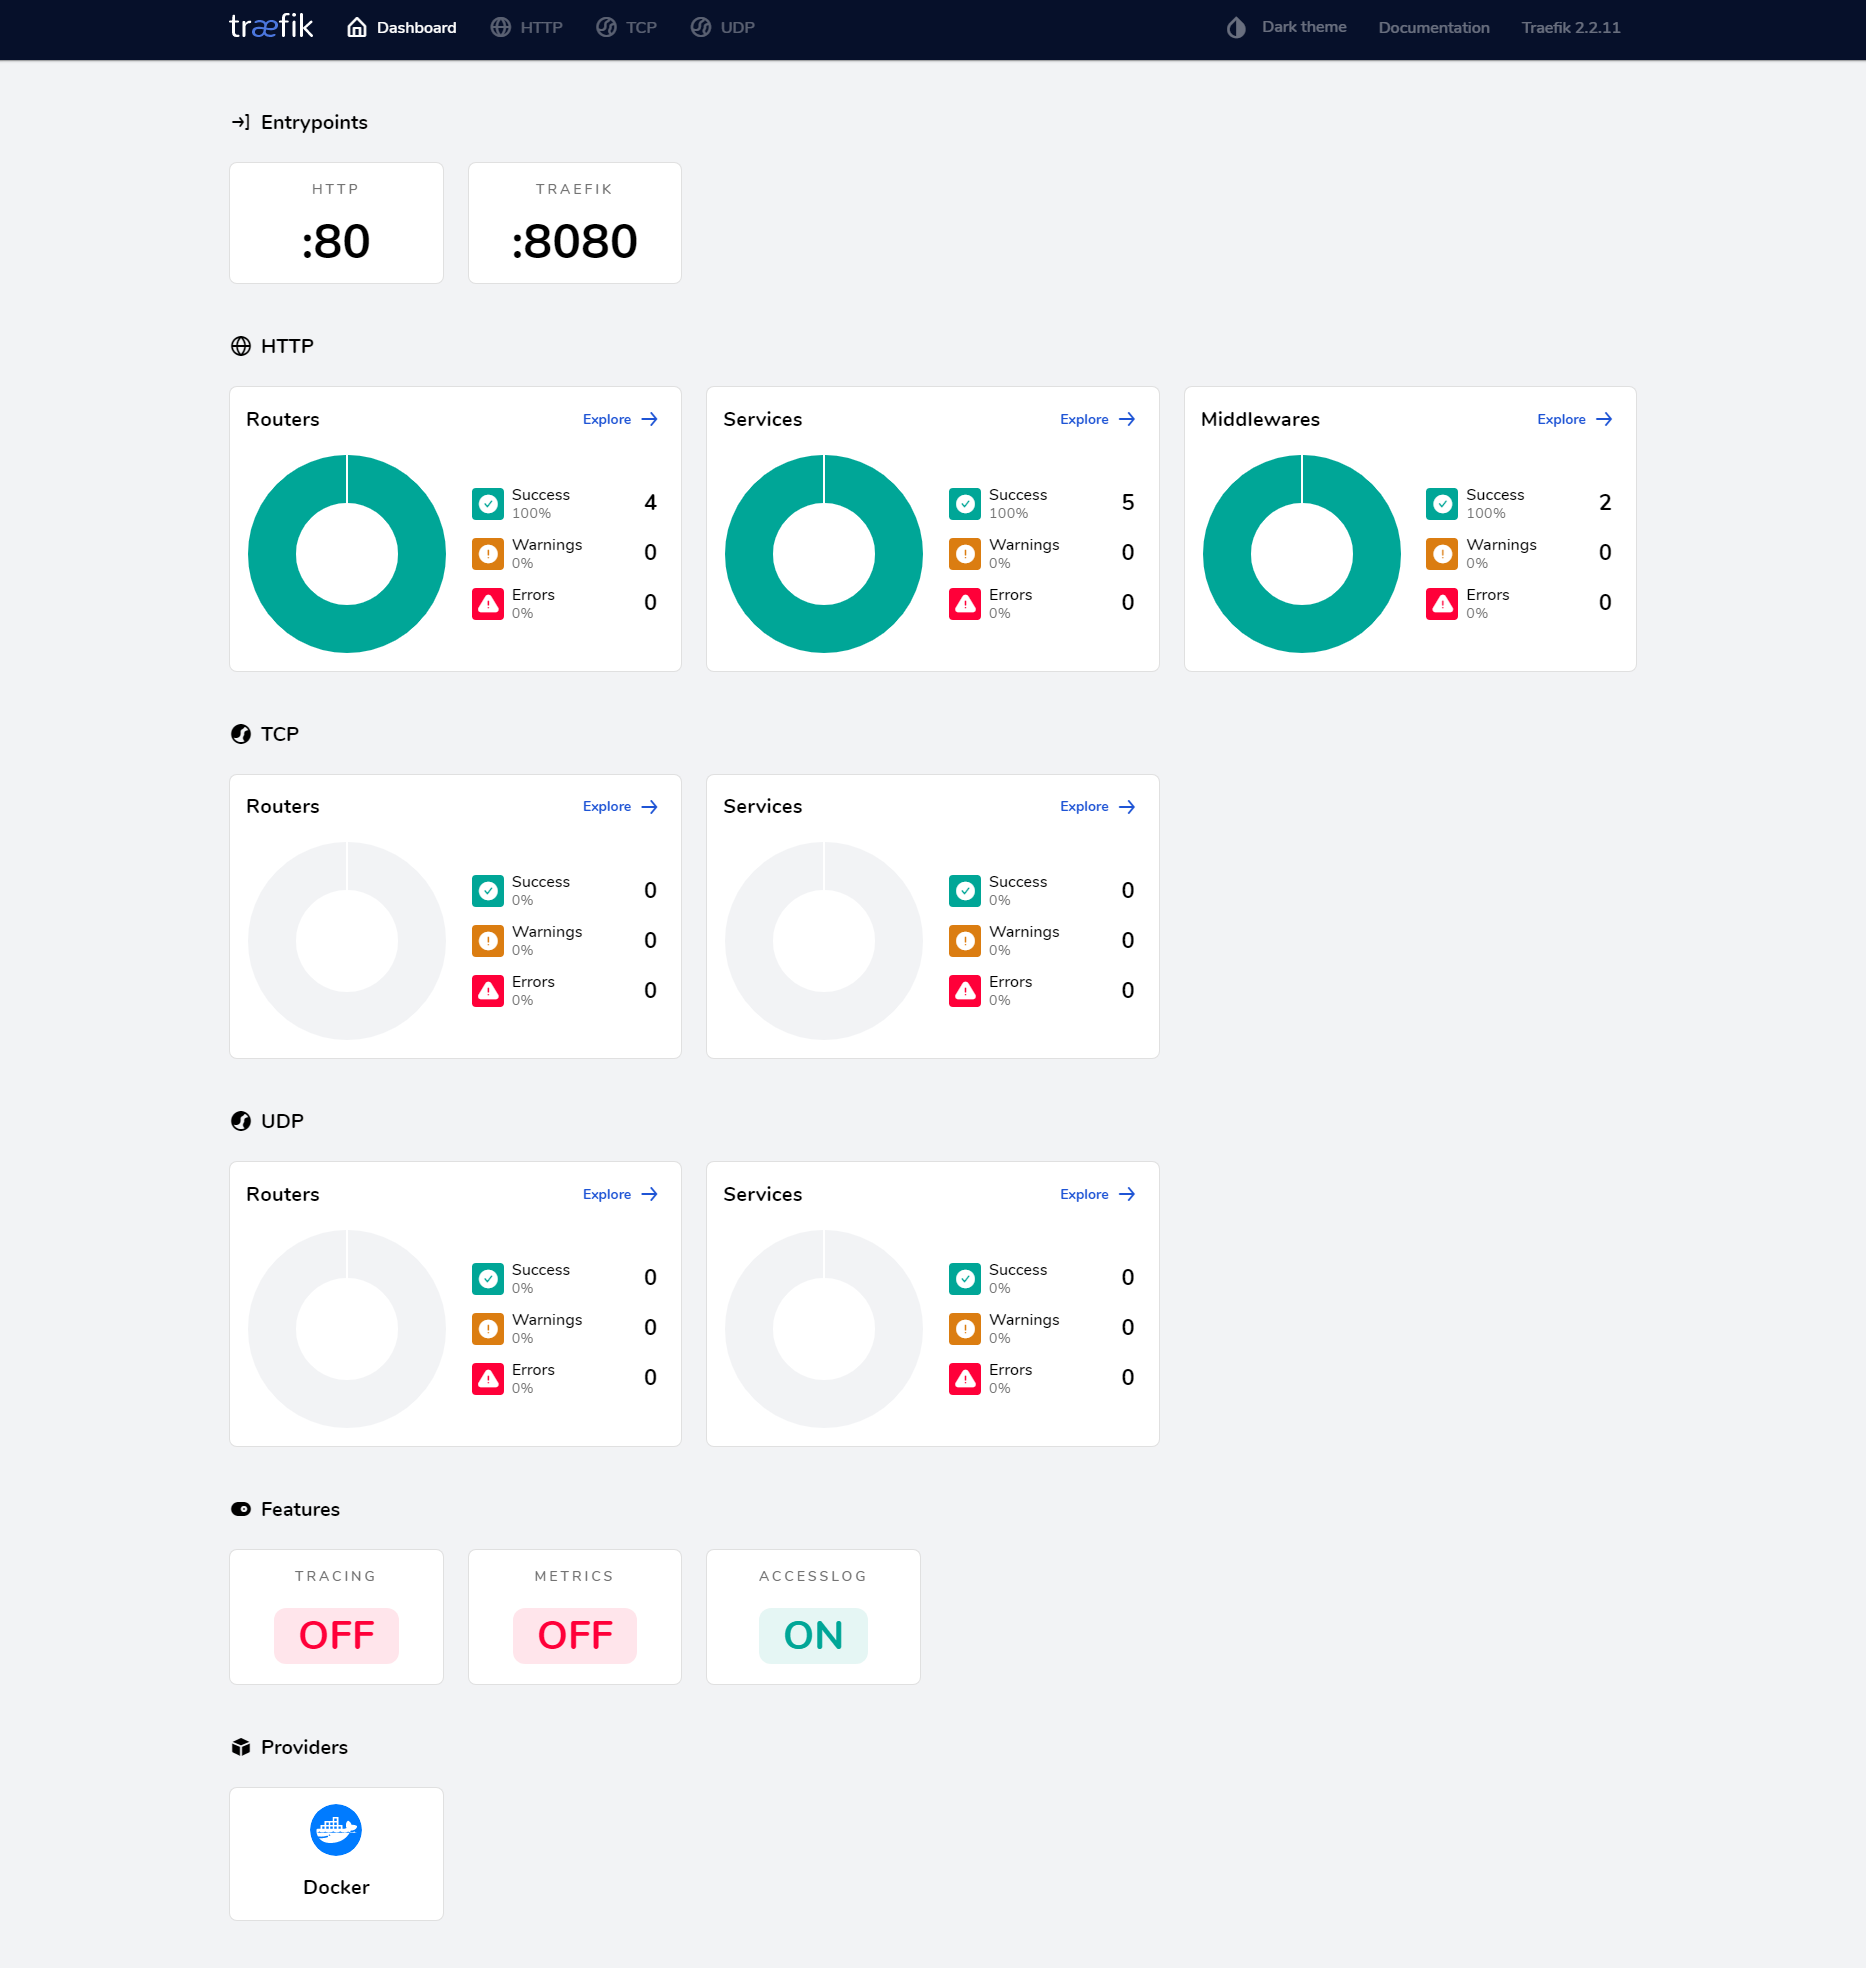
\includegraphics[scale=0.2]{TT/img/implementacion/Traefik dashboard.png}
    \caption{Dashboard de Traefik}
    \label{graphic:TraefikDashboard}    
\end{figure}

\subsection{Postgres}
Postgres es la herramienta elegida de base de datos para el sistema. Se eligió por ser 100\% OpenSource. También cuenta con una imagen de docker con la cual se ha configurado y trabajado para realizar el sistema.

\subsection{FastAPI}
Continuamos con FastApi, es una herramienta que ayuda a desarrollar API's de manera rápida basada en Python. Se usó una imagen de Python en su versión 3.9 en docker. A continuación se describirá el proceso de desarrollo de la API usando estas herramientas.

\subsubsection{Preparando entorno de desarrollo}
Para tener un control de los paquetes que vamos a usar, se ha elegido la herramienta Poetry, la cual nos ayuda a ordenar los paquetes a usar y que facilita la instalación de estos mismos en cualquier entorno en donde se despliegue el contenedor del sistema.

Primero crearemos nuestro proyecto usando Poetry para ir instalando las dependencias que se requieren para que la API funcione correctamente. Las dependencias son: 
\begin{itemize}
    \item fastapi = "\^0.68.1"
    \item SQLAlchemy = "\^1.4.25"
    \item uvicorn = "\^0.15.0"
    \item python-dotenv = "\^0.19.0"
    \item python-multipart = "\^0.0.5"
    \item python-jose = \{extras = [cryptography], version ="\^3.3.0"\}
    \item passlib = "\^1.7.4"
    \item pydantic = \{extras = [email], version ="\^1.8.2"\}
    \item alembic = "\^1.7.3"
    \item inflect = "\^5.3.0"
    \item bcrypt = "\^3.2.0"
    \item SQLAlchemy-Utils = "\^0.37.8"
    \item psycopg2-binary = "\^2.9.1"
    \item tenacity = "\^8.0.1"
    \item pytest = "\^6.2.5"
    \item mypy = "\^0.910"
    \item sqlalchemy-stubs = "\^0.4"
    \item flake8 = "\^3.9.2"
    \item autoflake = "\^1.4"
    \item isort = "\^5.9.3"
    \item black = "\^21.9b0"
    \item pytest-cov = "\^2.12.1"
    \item numpy = "\^1.21.4"
\end{itemize}

Los dependencias destacadas son: 
\begin{itemize}
    \item \textbf{Fastapi: }Es la dependencia que contiene el framework con el que vamos a trabajar.
    \item \textbf{SQLAlchemy: }Es una herramienta que permite trabajar las bases de datos como \gls{ORM} en Python.
    \item \textbf{Uvicorn: }Es un servidor ASGI rápido. Uvicorn se basa en uvloop y httptools y es un miembro importante del ecosistema asincrónico de Python.
    \item \textbf{Alembic: }es una herramienta de migración de bases de datos escrita por el autor de SQLAlchemy que permite versionar las bases de datos, en otras palabras, tener un historial de los cambios que se vayan realizando a la base de datos, ejemplo: cambiar el nombre de una tabla, el nombre de uno o varios atributos, las especificaciones de estos, etc.
    \item \textbf{Psycopg2-binary: }es el adaptador de base de datos PostgreSQL para el lenguaje de programación Python.
\end{itemize}

Poetry ofrece la opción de crear un entorno virtual en Python, pero como se ha configurado una imagen de Python para el desarrollo del sistema, no es necesario crear un entorno virtual para la instalación de los paquetes vistos anteriormente.

\subsubsection{Estructura de la API}
Continuemos con la estructura de la API, en esta sección se describirá las carpetas y que es lo que almacenan. En la carpeta backend se localiza el archivo de configuración de docker, con el cual se configura el entorno del contenedor y ejecutar algunos scripts. 

\textbf{Nivel 1 y 2}

En la carpeta \textit{app} que se muestra en la figura \ref{graphic:carpetasapi1} hay mas carpetas, que se visualizan en la figura \ref{graphic:carpetasapi2}. Adentro se localizan la carpeta \textit{alembic}: en esta carpeta se encuentra la herramienta que actúa como versionador de bases de datos; en la carpeta scripts hay archivos que corrigen el formato de los archivos python así como realizar test básicos del sistema; lo siguiente por explicar son los archivos que se encuentran en la raíz de \textit{app}, los cuáles son archivos de configuración para la base de datos y la lista de paquetes administrada por poetry para el entorno de trabajo; por último se encuentra otra carpeta igualmente \textit{app}, en ella se encuentran los archivos de python que conforman el sistema.

\begin{figure}[!htb]
    \centering
    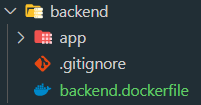
\includegraphics[scale=1]{TT/img/implementacion/carpeta-api-1.png}
    \caption{Carpetas de la API - Parte 1}
    \label{graphic:carpetasapi1}    
\end{figure}

\begin{figure}[!htb]
    \centering
    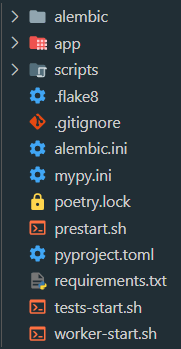
\includegraphics[scale=1]{TT/img/implementacion/carpeta-api-2.png}
    \caption{Carpetas de la API - Parte 2}
    \label{graphic:carpetasapi2}    
\end{figure}

\textbf{Nivel 3}

Continua la explicación de la carpeta \textit{app}, esta carpeta contiene los archivos del proyecto, se muestran en la figura \ref{graphic:carpetasapi3}. Iniciamos con la carpeta models, en esta carpeta se encuentran los archivos donde se han definido los modelos de la base de datos, cada tabla de la base de datos se define como una clase y dentro de cada clase se definen los atributos de las tablas, sus relaciones, tipos de atributos y características como que sea nulo, único, sea llave primaria o llave foránea, etc. Esto se muestra en la figura \ref{graphic:user_model}.

\begin{figure}[!htb]
    \centering
    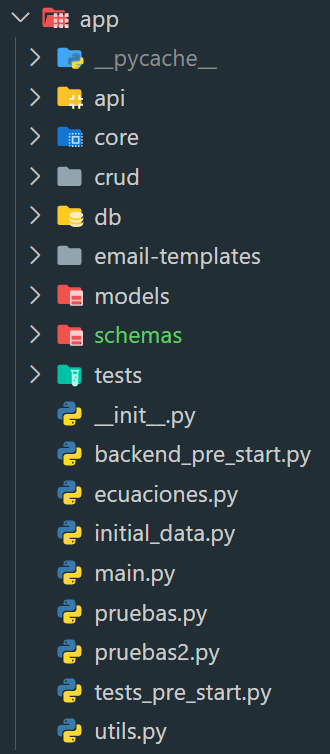
\includegraphics[scale=.9]{TT/img/implementacion/carpeta-api-3.png}
    \caption{Carpetas de la API - Parte 3}
    \label{graphic:carpetasapi3}    
\end{figure}

\begin{figure}[!htb]
    \centering
    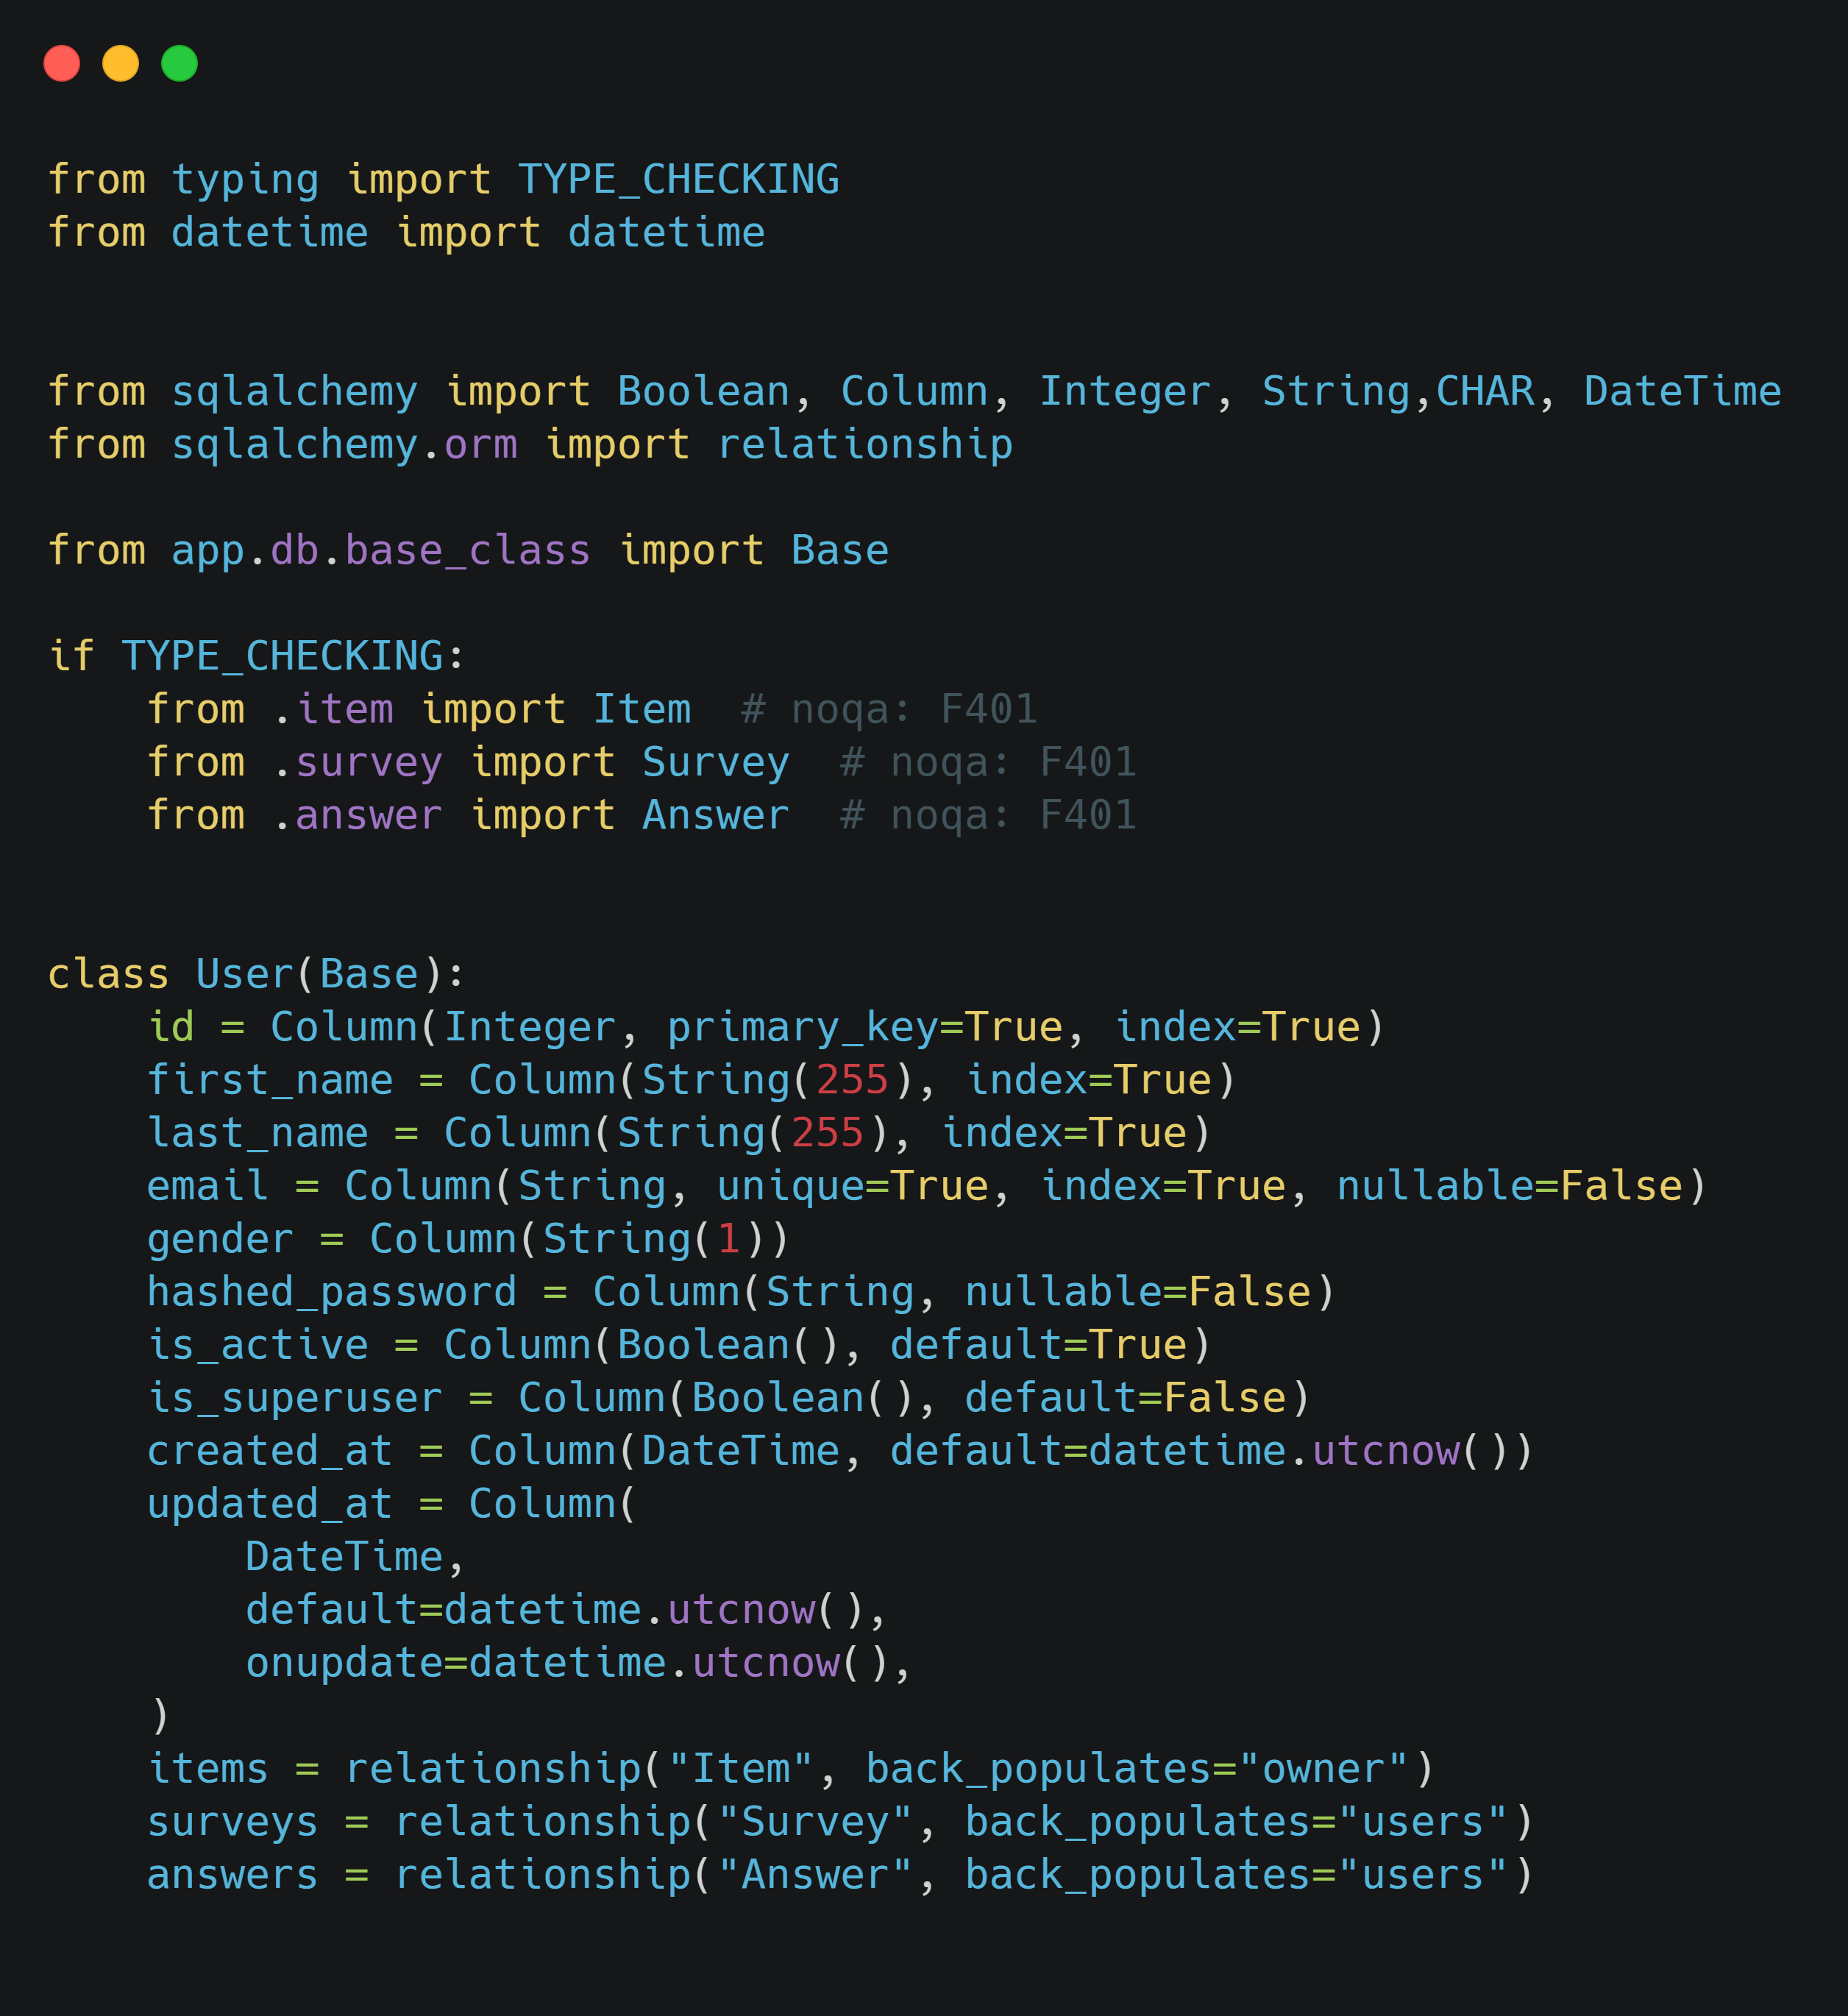
\includegraphics[scale=.15]{TT/img/implementacion/user-model.png}
    \caption{Modelo de usuario}
    \label{graphic:user_model}    
\end{figure}

Continuamos con la carpeta \textit{schemas}, dentro de esta carpeta tendremos los esquemas de los modelos de la base de datos, estos archivos nos ayudan a tener una estructura sobre los datos que son los accesibles por el usuario y cuales son los que el sistema creará de manera automática, así como el tipo de dato que van a aceptar, esto nos ayuda a que solo entren los tipos de datos que son requeridos por la base de datos lo que añade una capa de seguridad, ya que si se envían datos que no están definidos en las clases simplemente no se podrá guardar o modificar los datos guardados en la base de datos. También se define que datos son los que van a ser creados y actualizados, en la figura \ref{graphic:user_schema} donde se muestra el esquema para la tabla usuario.

\begin{figure}[!htb]
    \centering
    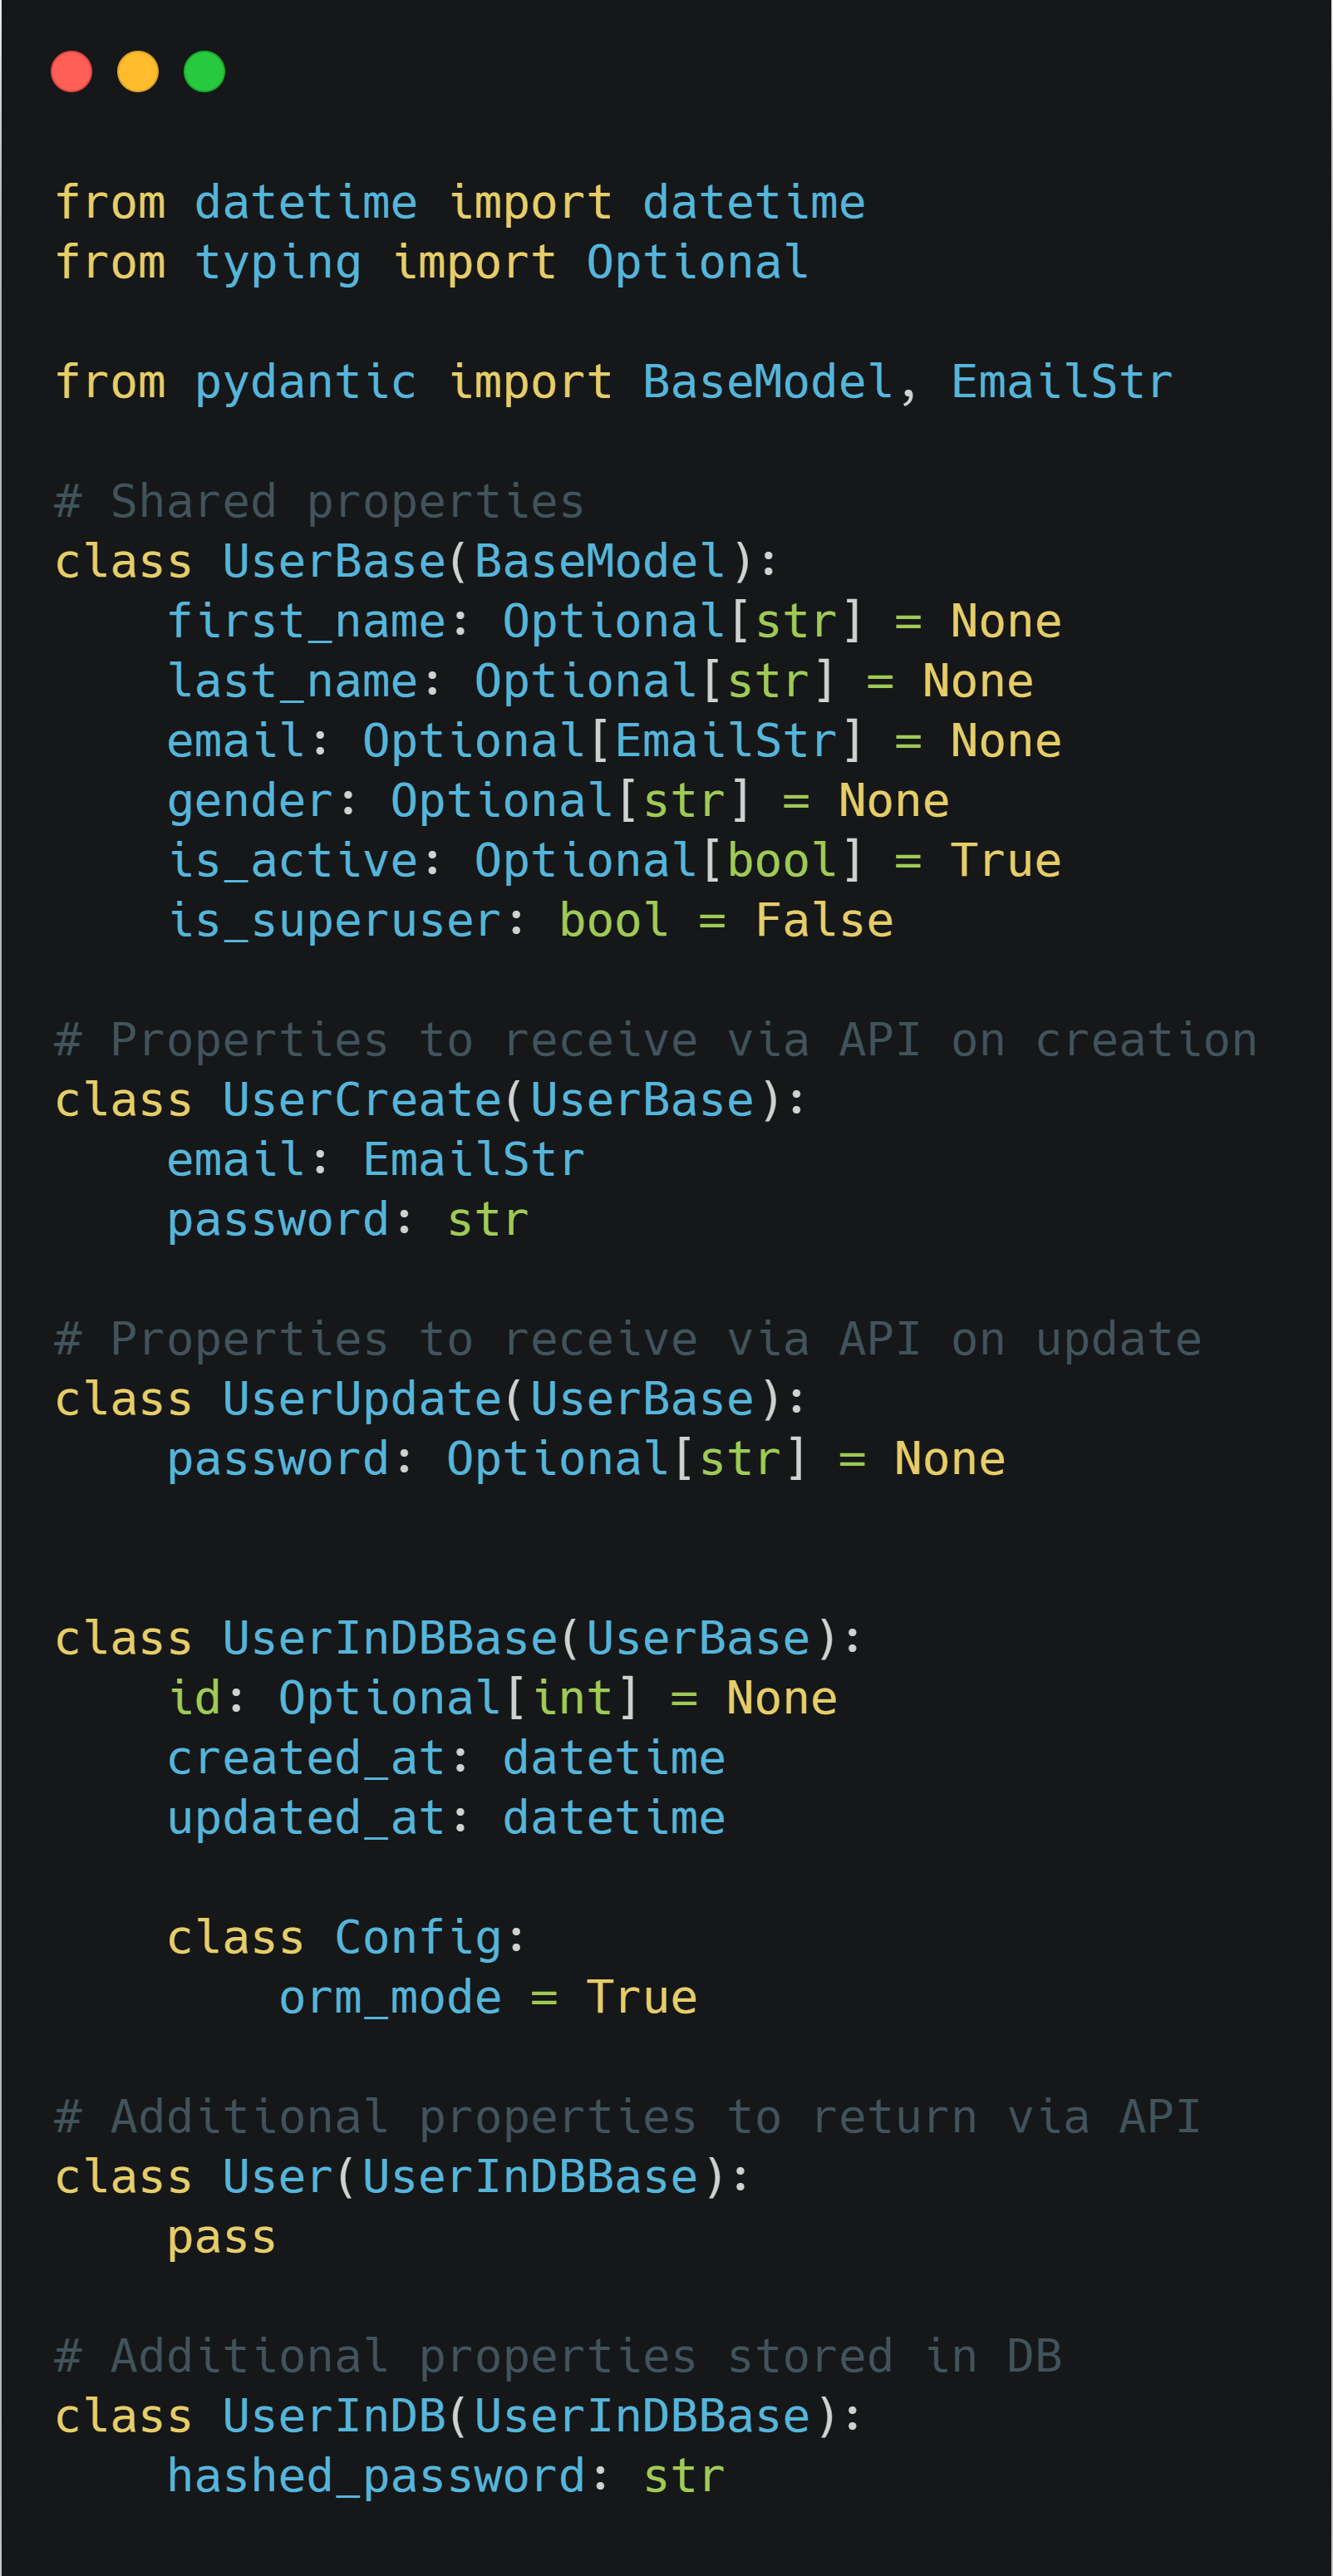
\includegraphics[scale=.15]{TT/img/implementacion/schema-user.png}
    \caption{Esquema de usuario}
    \label{graphic:user_schema}    
\end{figure}

La siguiente carpeta a presentar es \textit{crud}, en esta carpeta se encuentra el CRUD de cada tabla de la base de datos, se define un CRUD base, donde se definen las funciones básicas de crear, leer, actualizar y eliminar un elemento de la base de datos. Para complementar las funciones básicas, se han creado archivos para cada tabla en la base de datos, ya que se han requerido otras funciones, por ende, estos archivos heredan las funciones básicas ya mencionadas anteriormente, algunos ejemplos son los que se encuentran en el CRUD de usuario que se muestran en la figura \ref{graphic:user_crud} donde se aprecian funciones para buscar usuarios mediante el correo electrónico, autenticar un usuario u obtener si el usuario se encuentra activo o es un súper-usuario.

\begin{figure}[!htb]
    \centering
    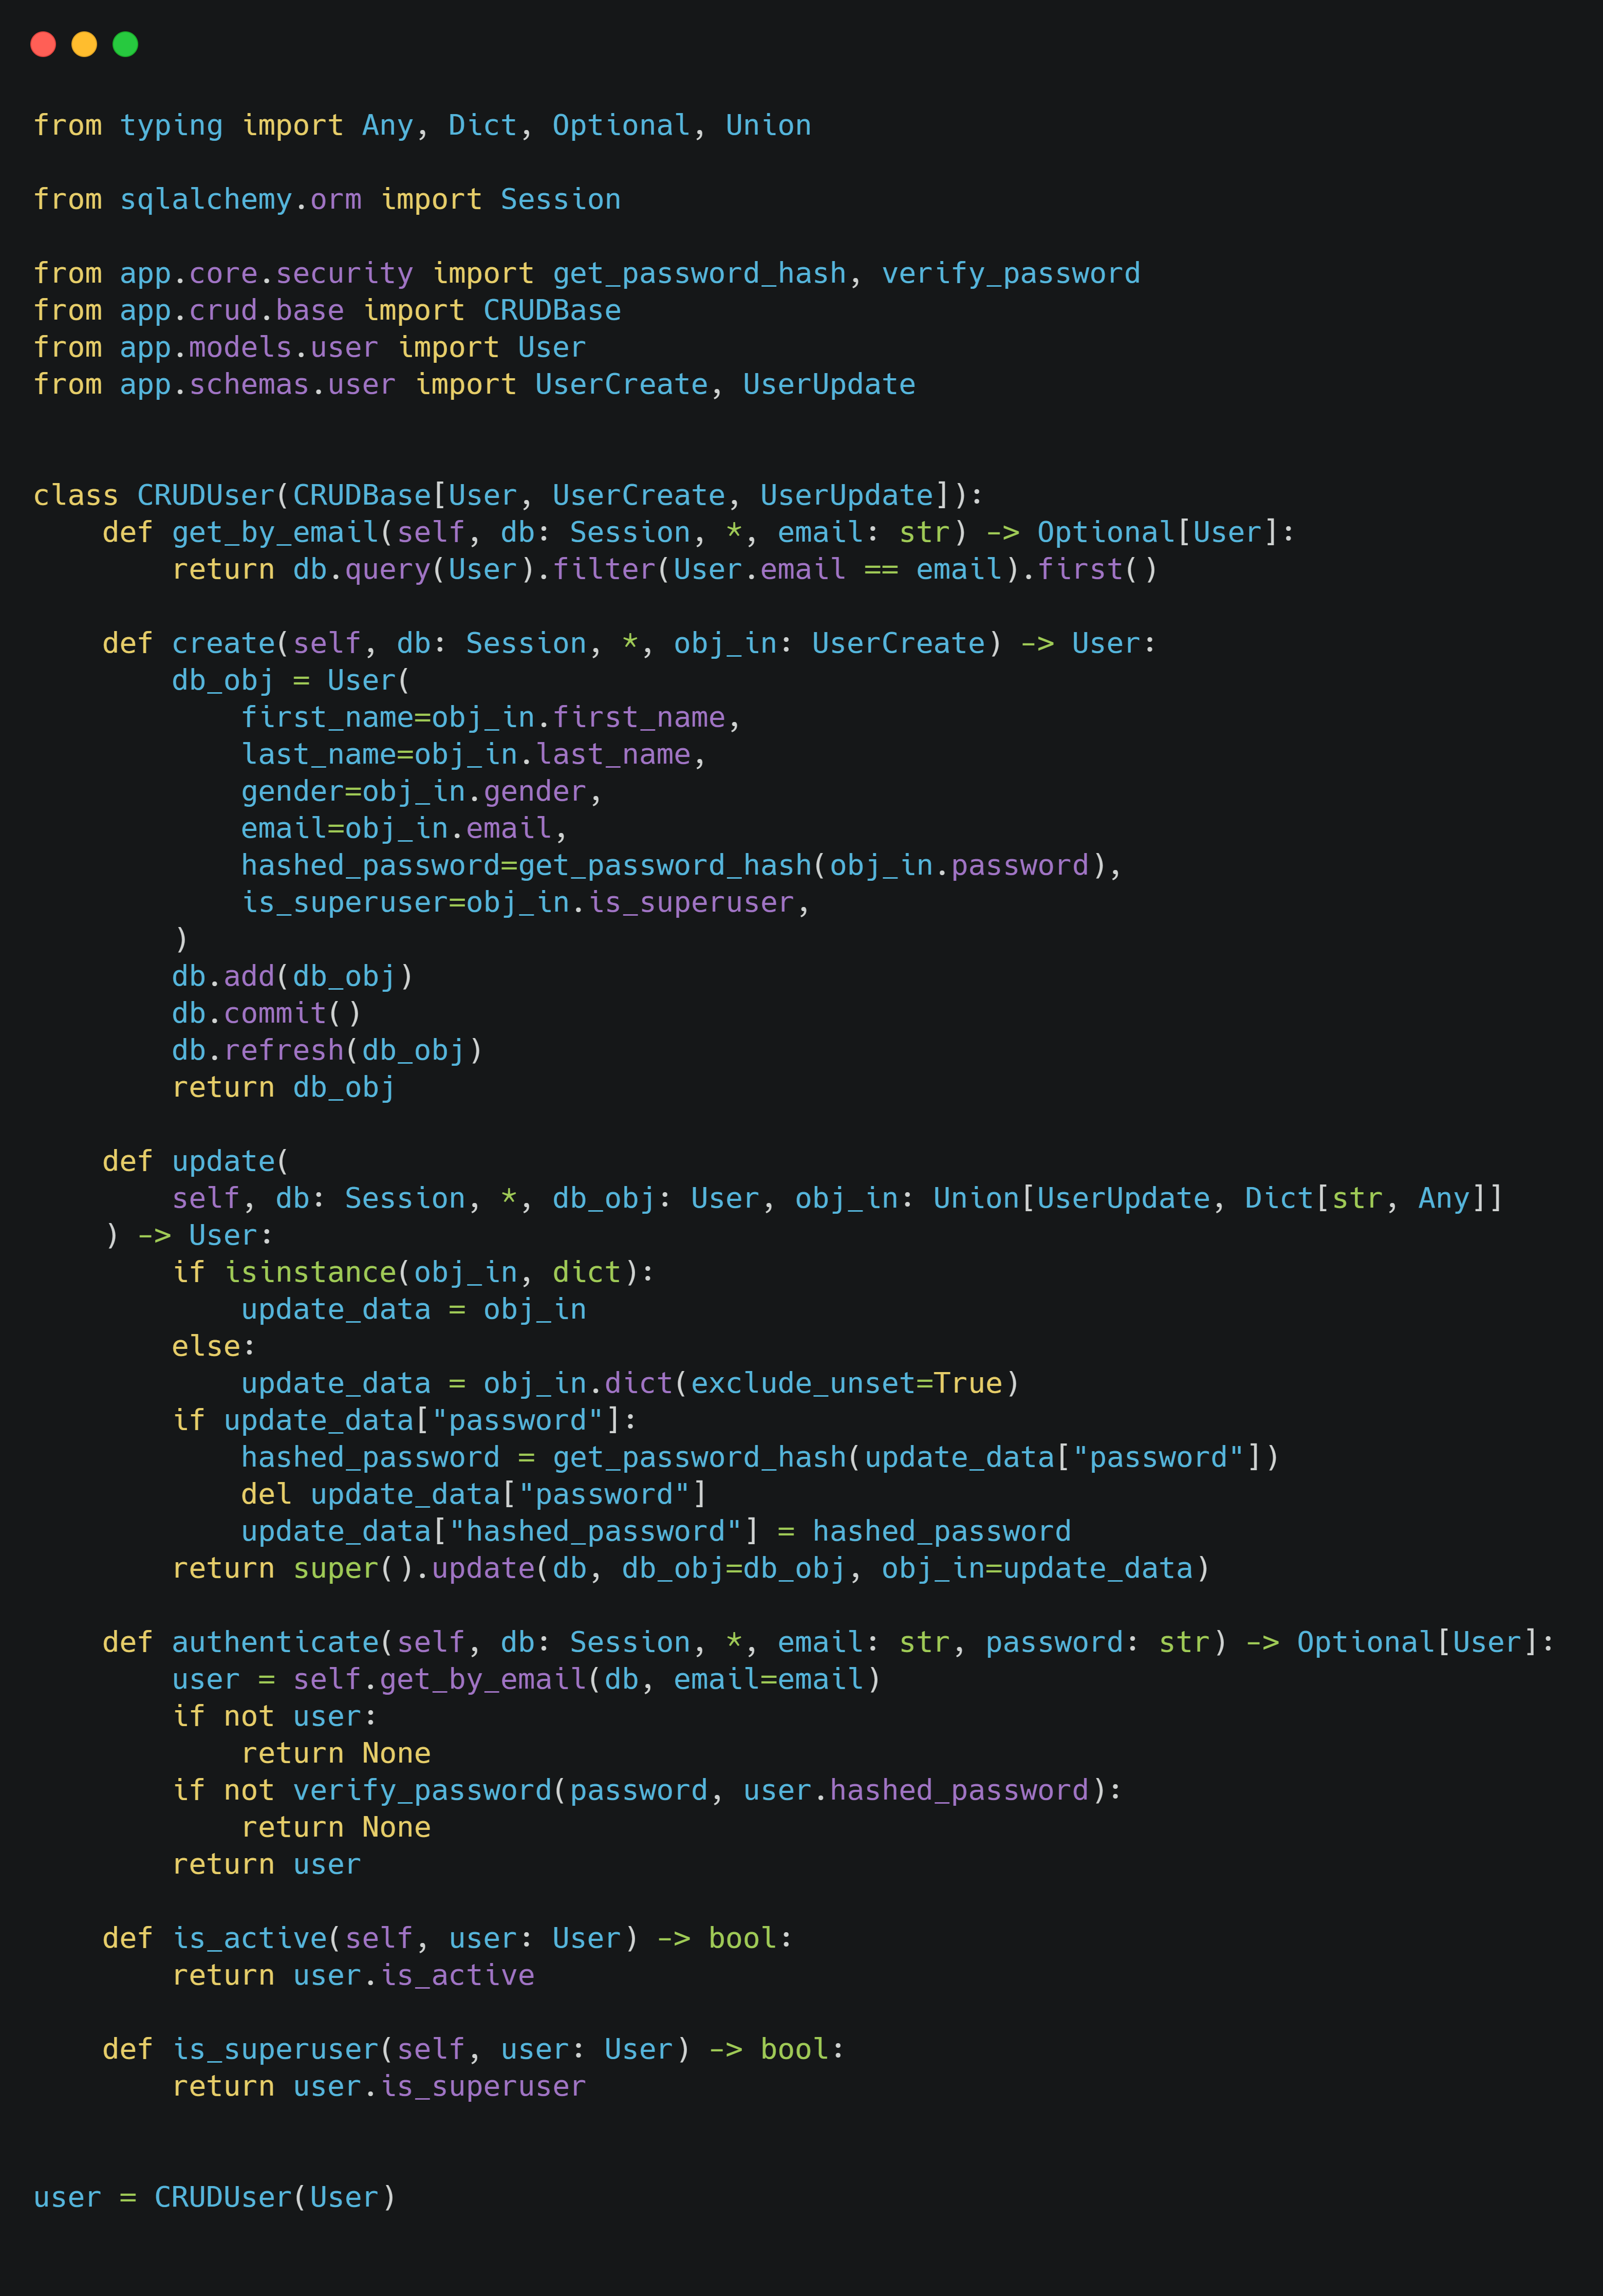
\includegraphics[scale=.10]{TT/img/implementacion/crud_user.png}
    \caption{CRUD de usuario}
    \label{graphic:user_crud}    
\end{figure}

Una de las carpetas esenciales es la llamada \textit{db}, en esta se encuentra la conexión con la base de datos y los archivos que gestiona el arranque de la base de datos, la conexión con el sistema gestor de la base de datos, en este caso postgres, los modelos que se usarán para la base de datos y que alembic y sqlalchemy necesitan para crear y modificar la base de datos en postgres, así como la creación del primer súper-usuario si se ejecuta el contenedor por primera vez.

Por otro lado, tenemos a la carpeta \textit{core}, aquí es donde se encuentran los archivos que se encargan de la seguridad y la configuración del servidor que se ejecutará en el contenedor, algunas de las funciones que se pueden encontrar en estos archivos son: la dirección que sigue del dominio para acceder a los endpoints de la API, el algoritmo de encriptación que en este caso es \textbf{HS256}, la llave de encriptación que es hexadecimal de 32 bits, la duración del token, verificar contraseñas o crear tokens, etc.

A continuación se describe la carpeta \textit{api}, dentro de esta carpeta se localizan los endpoints de la API y funciones importantes como se aprecia en la figura \ref{graphic:deps}, en donde se aprecia las funciones para obtener estados del usuario que son necesarios para validar las peticiones que se harán a la base de datos. En los archivos que se pueden encontrar dentro de esta carpeta, están los responsables de realizar las peticiones HTTP a la base de datos \textit{(Get, Put, Post, Delete)}. En las figuras \ref{graphic:user_endpoint_1} y \ref{graphic:user_endpoint_2} se detallan todas las funciones para las peticiones HTTP que corresponden al usuario, también se pueden definir los estados de error en caso de que la petición que se realice falle.

\begin{figure}[!htb]
    \centering
    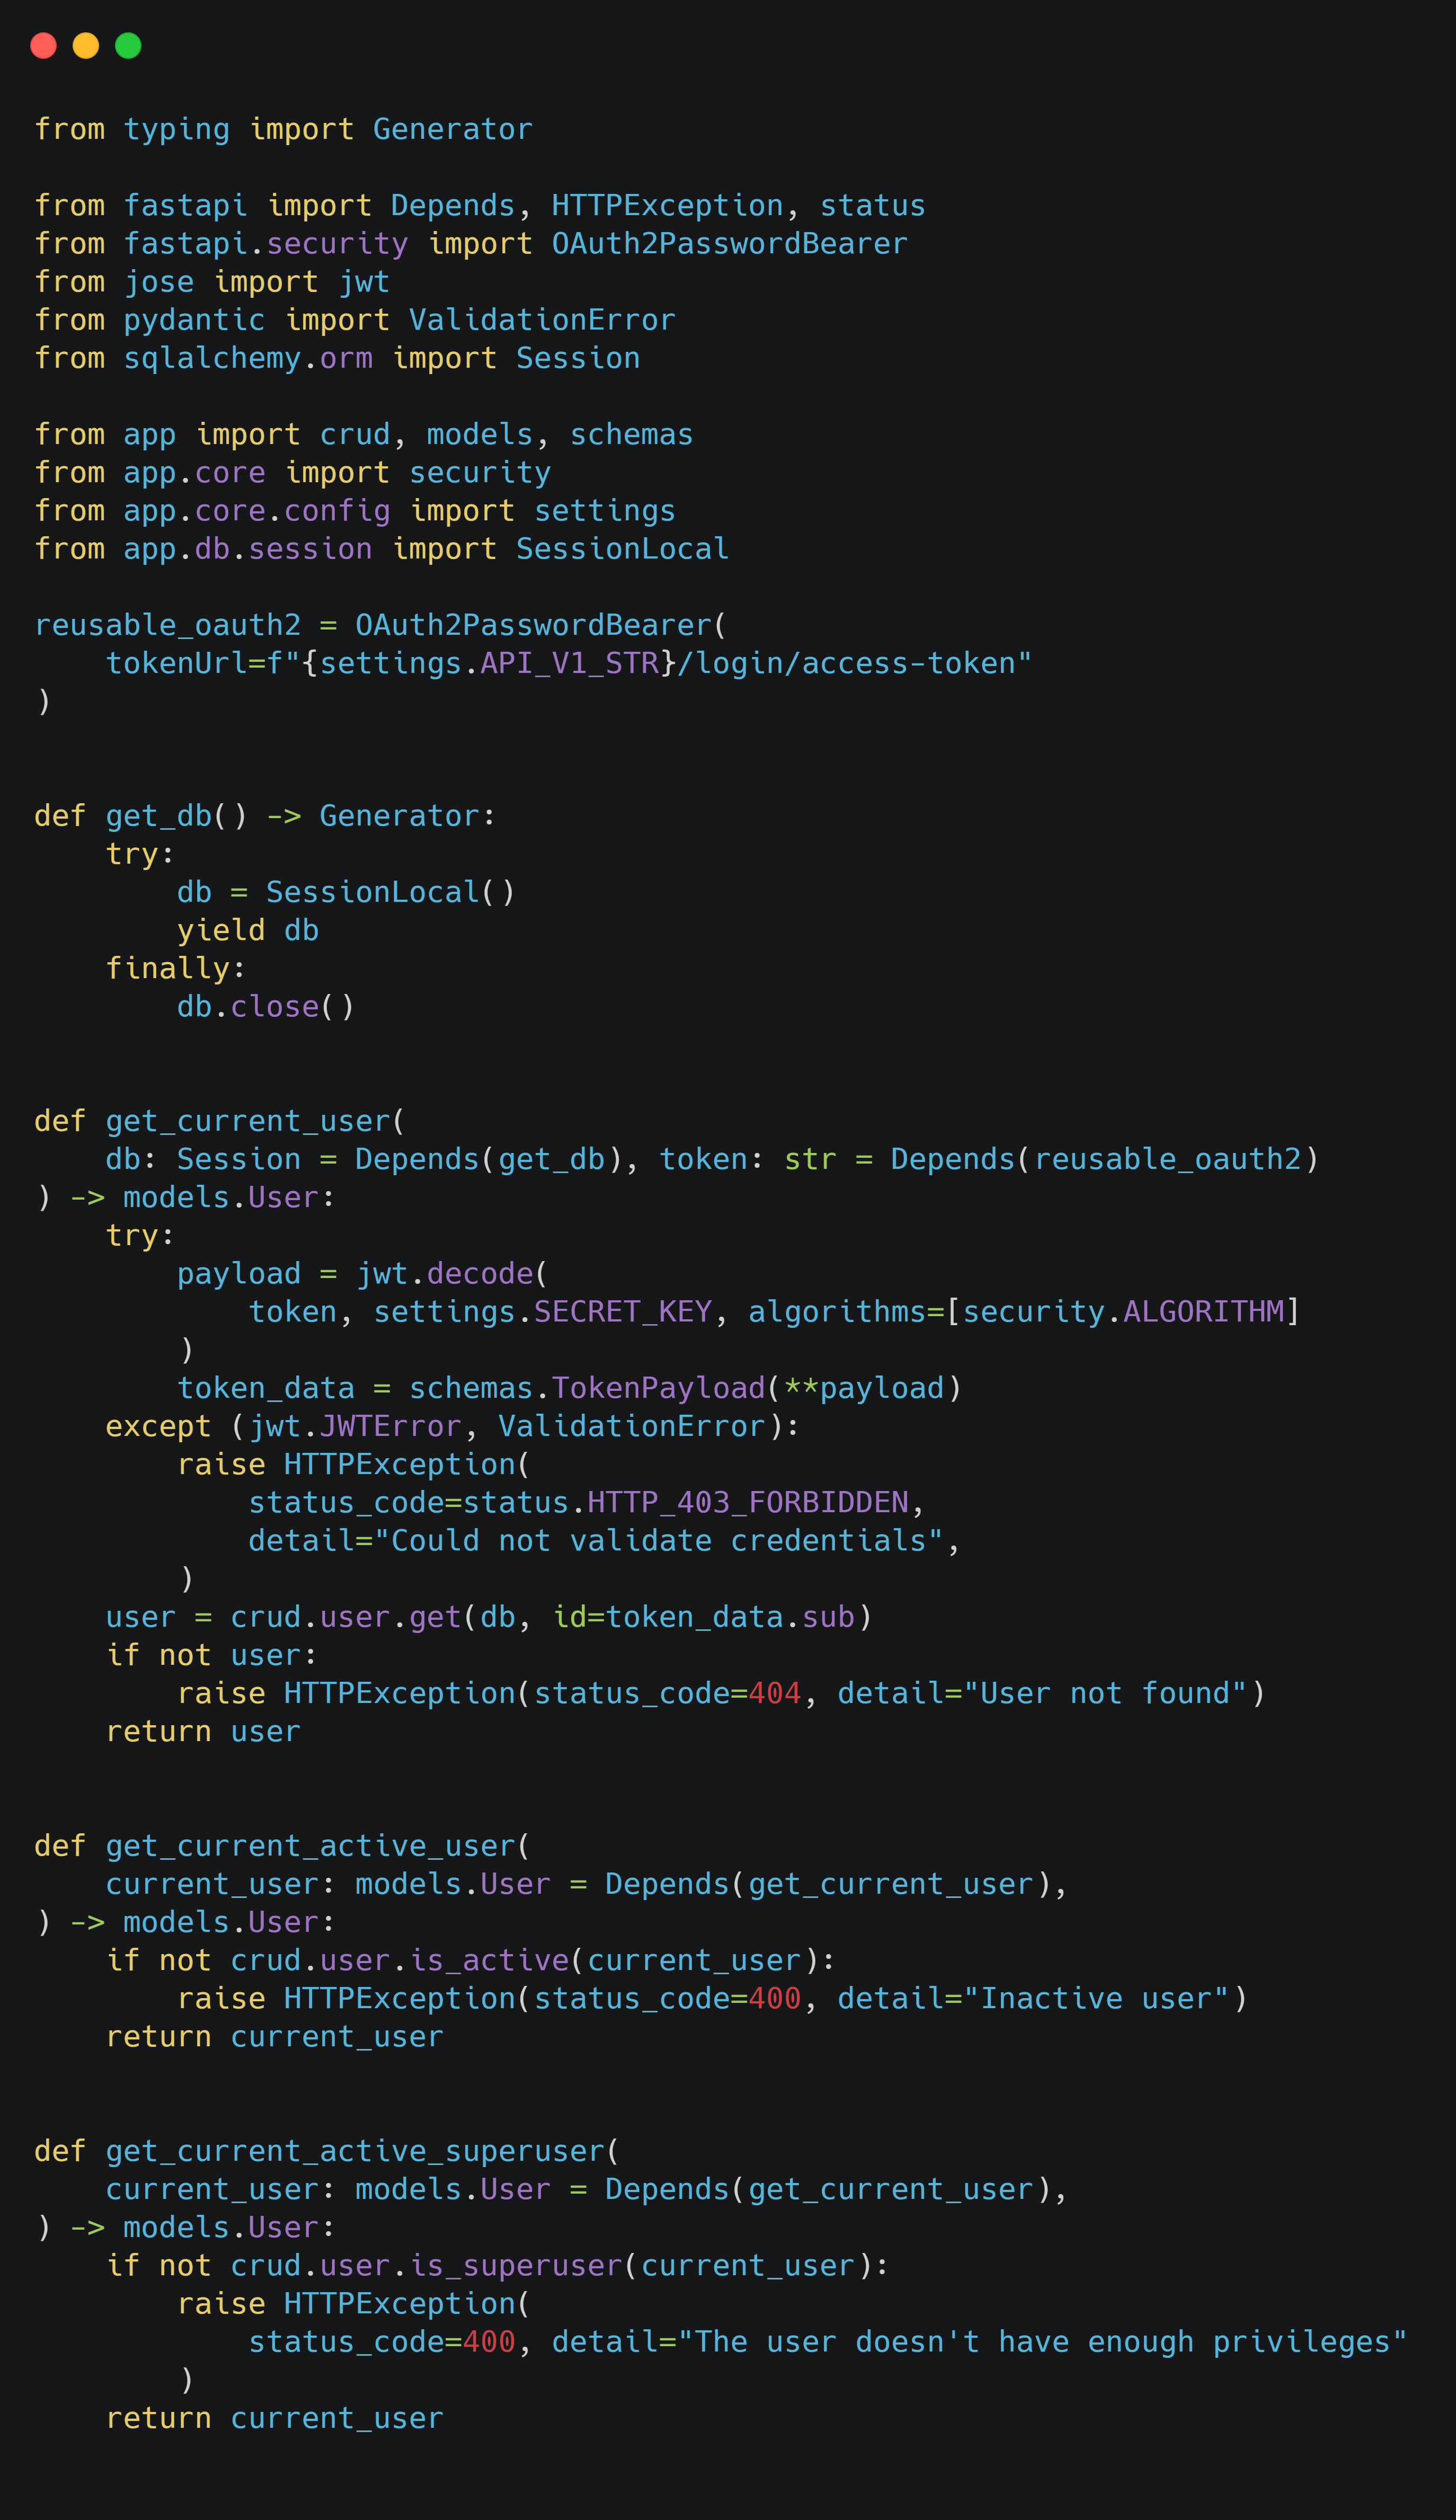
\includegraphics[scale=.10]{TT/img/implementacion/deps.png}
    \caption{Funciones para obtener estados del usuario}
    \label{graphic:deps}    
\end{figure}

\begin{figure}[!htb]
    \centering
    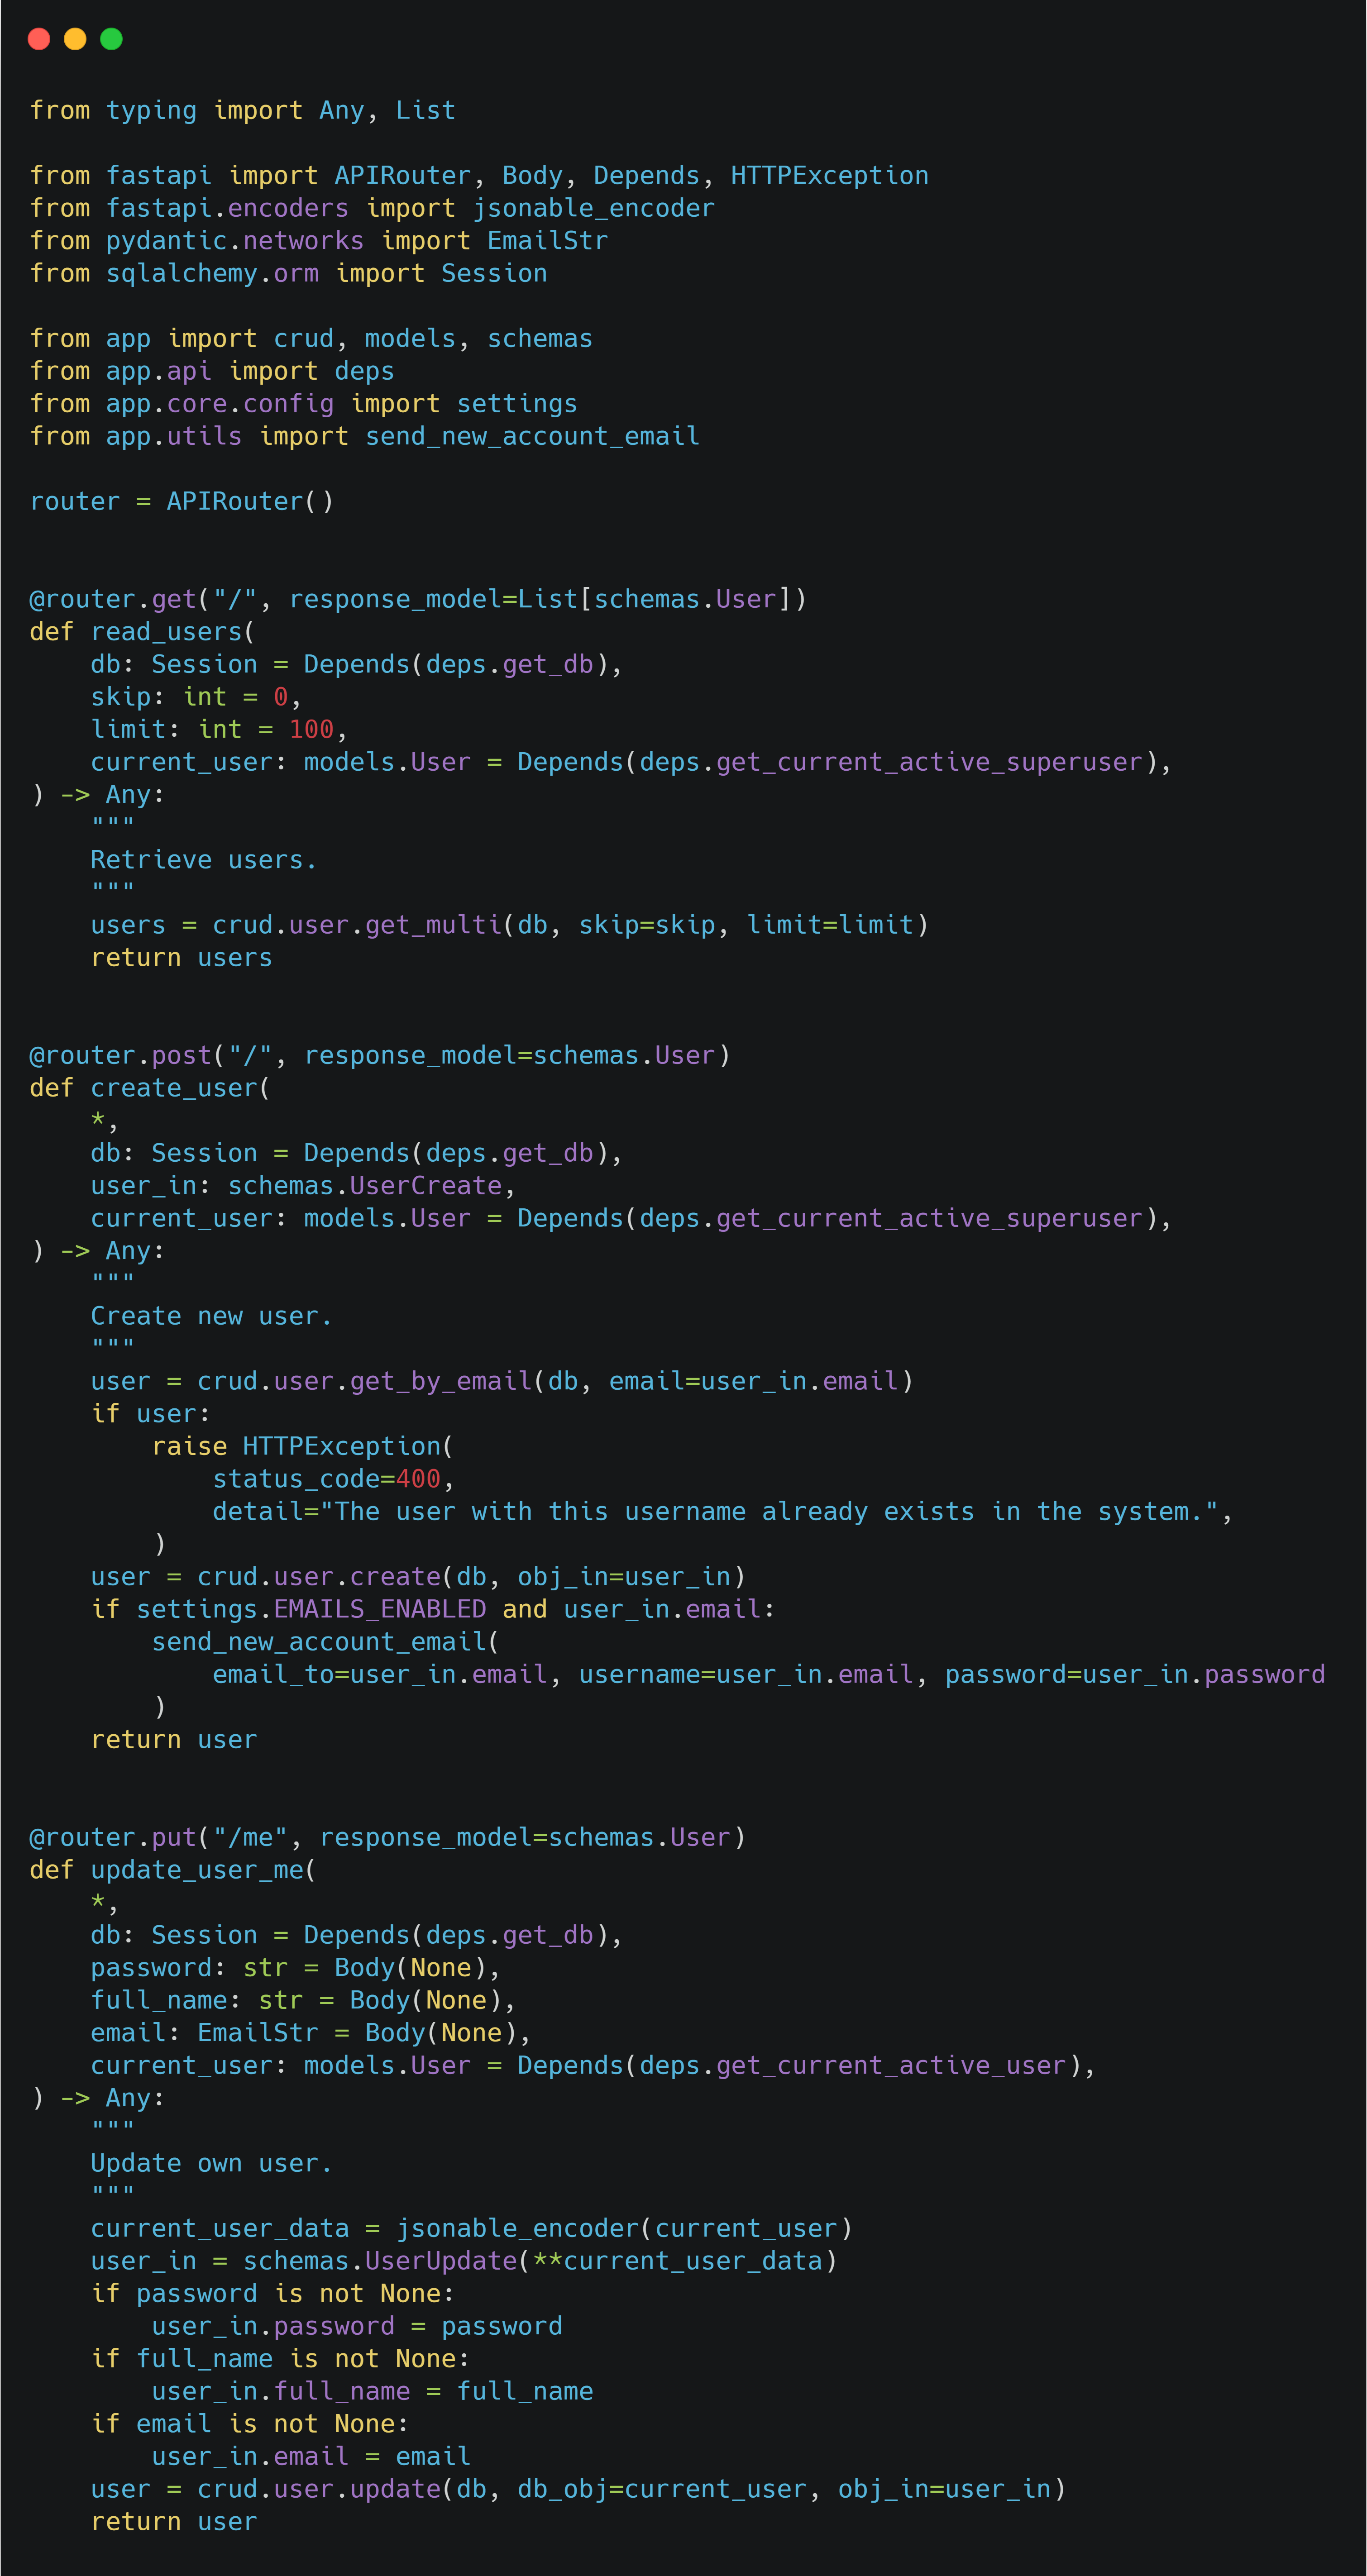
\includegraphics[scale=.10]{TT/img/implementacion/user_endpoint_1.png}
    \caption{Funciones para realizar peticiones de la API - Parte 1}
    \label{graphic:user_endpoint_1}    
\end{figure}

\begin{figure}[!htb]
    \centering
    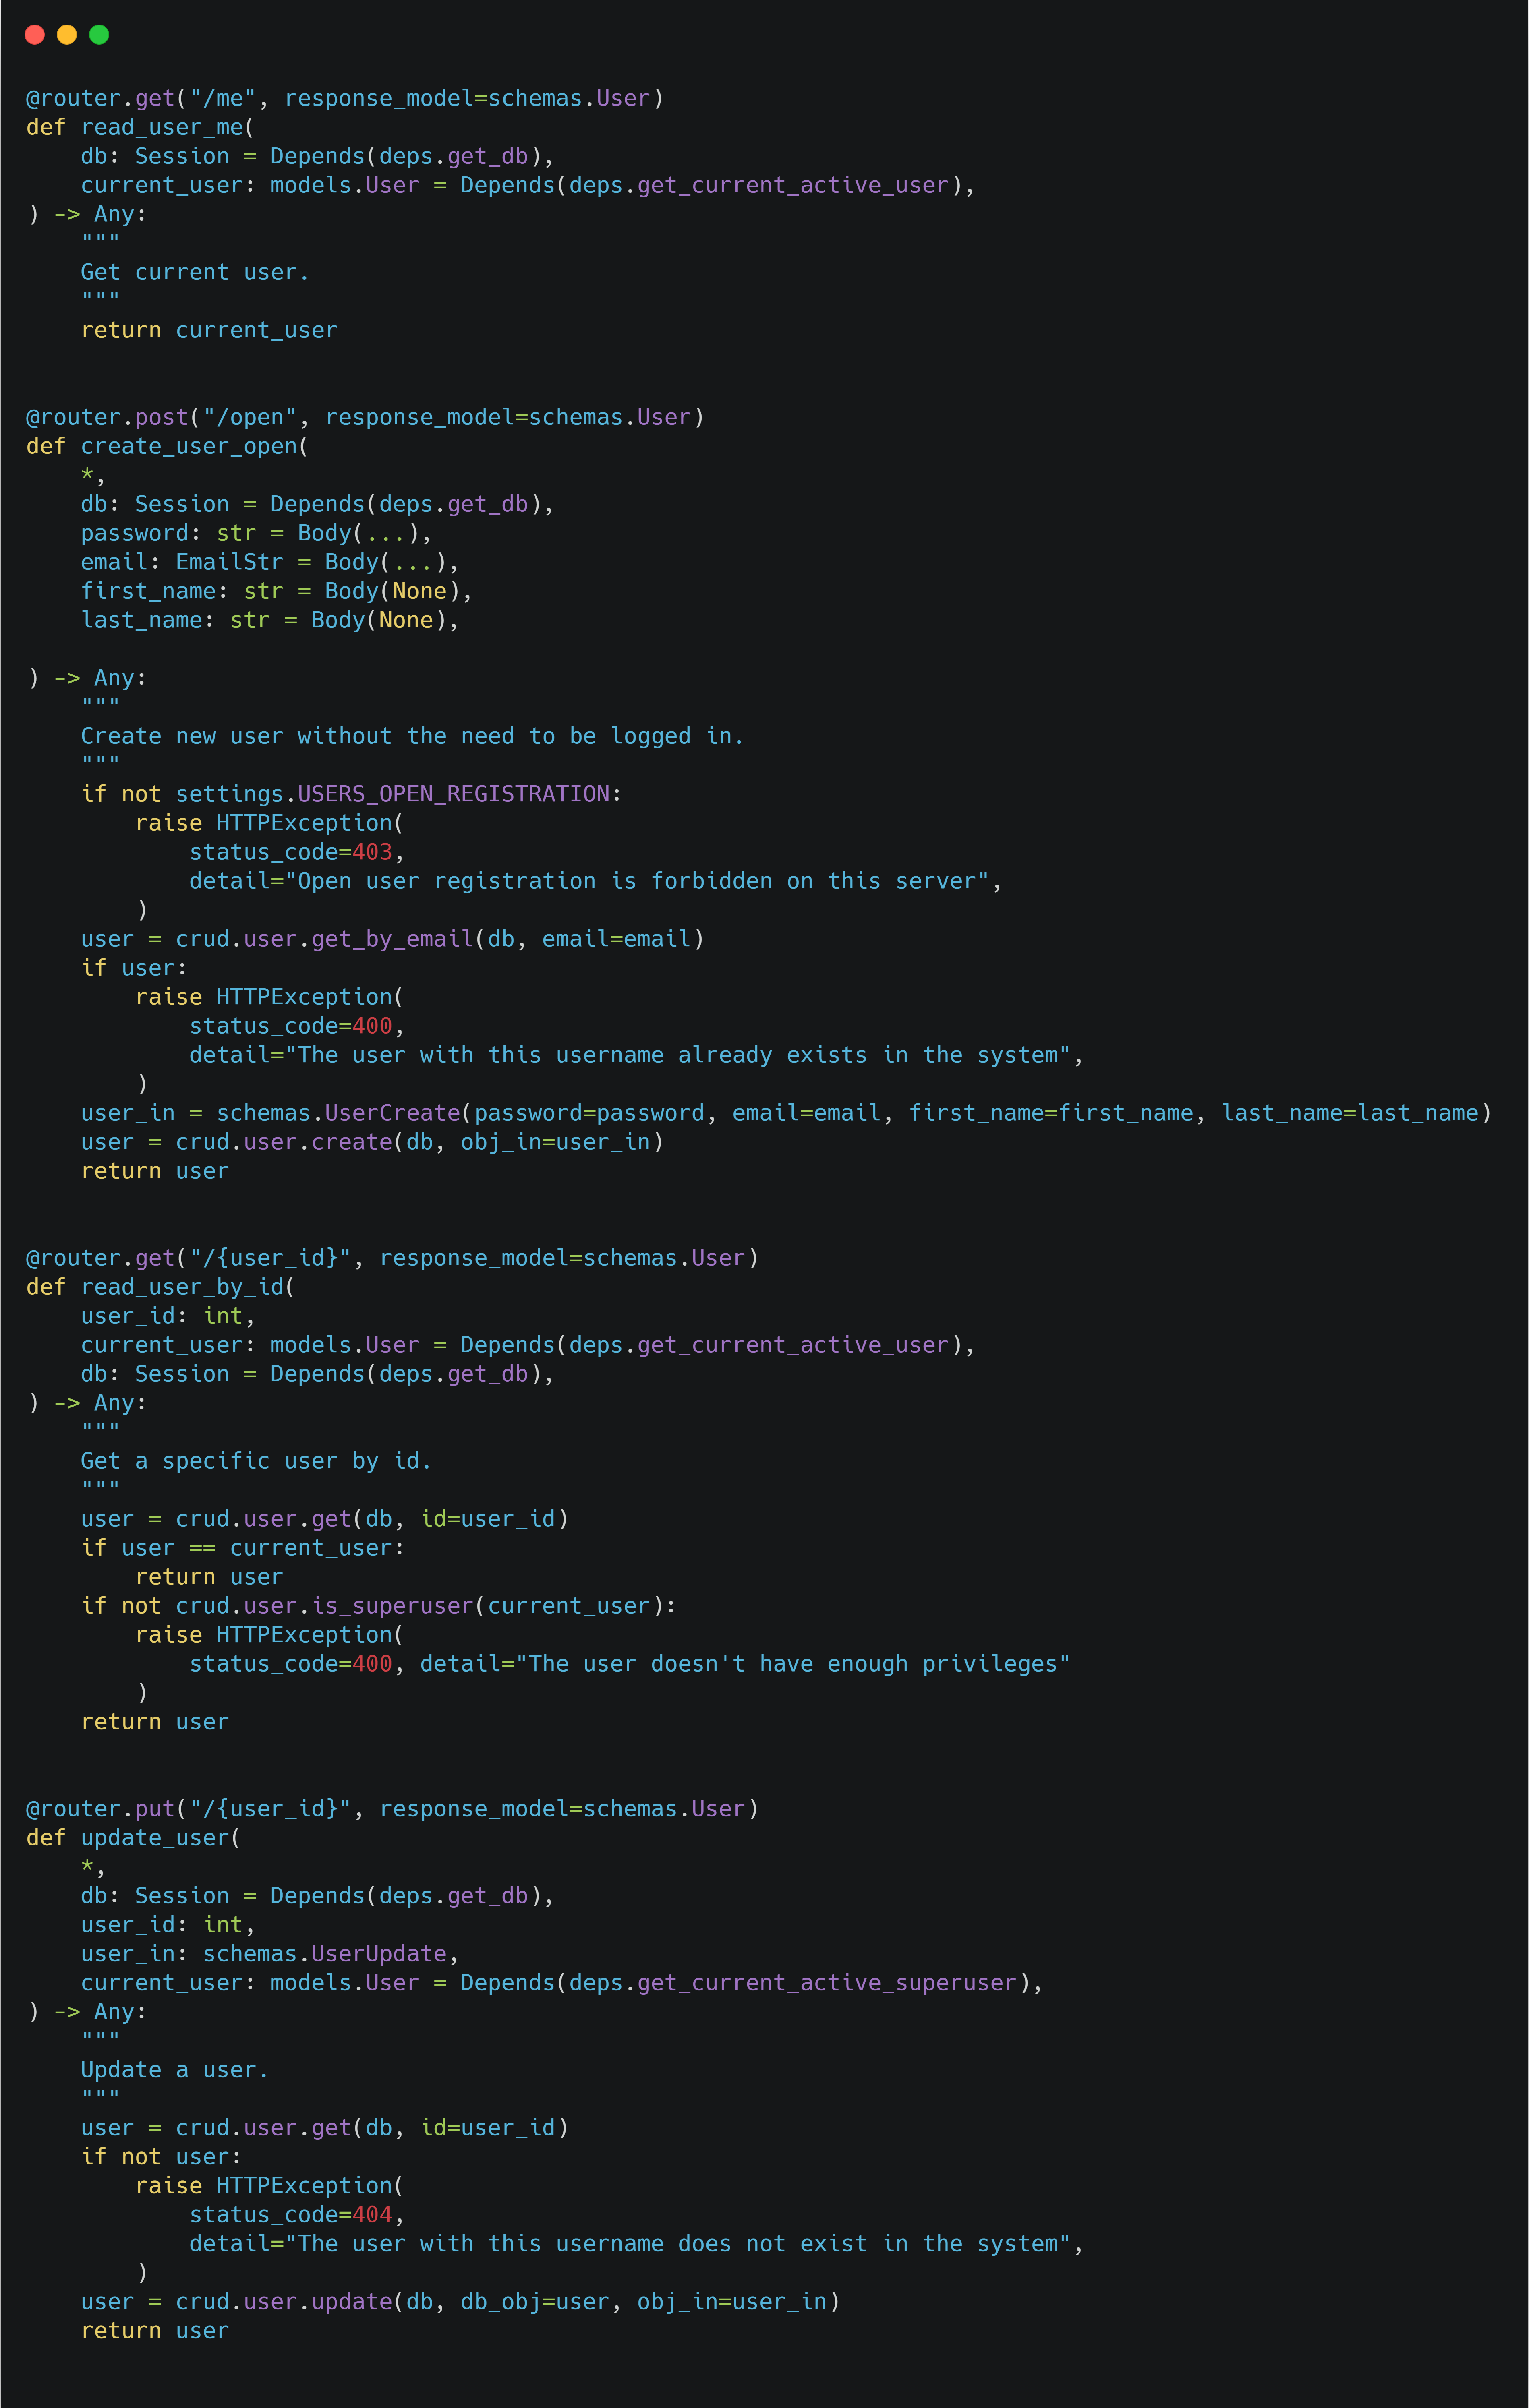
\includegraphics[scale=.10]{TT/img/implementacion/user_endpoint_2.png}
    \caption{Funciones para realizar peticiones de la API - Parte 2}
    \label{graphic:user_endpoint_2}    
\end{figure}

Para finalizar esta sección se describirán las carpetas y archivos faltantes. Primero, describimos la carpeta \textit{email-templates}, en esta carpeta se encuentran los archivos que tienen el diseño para enviar correos electrónicos para la creación de cuenta nueva, restablecer la contraseña y un template de prueba. En segundo lugar, la carpeta \textit{tests} almacena los archivos para realizar pruebas de funcionamiento a la API. Por último, pero no menos importante, los archivos que están en app, la mayoría de estos han sido creados para poder ejecutar la API en la imagen del contenedor de python, así como inicializar las pruebas a la API y archivos que tienen funciones variadas para las pruebas o para realizar cálculos que son necesarios para las predicciones del sistema.

\clearpage
\subsubsection{Oauth2}
En las secciones anteriores se ha hablado un poco de la seguridad del sistema con el uso de token y la generación de una llave del sistema basada en el algoritmo HS256, con ello podemos abordar el manejo del acceso a los endpoints del sistema, para esto se ha usado un protocolo de autorización que viene integrado en FastApi, hablamos del protocolo de autorización OAuth2. Este es un estándar abierto para las API's consiste en compartir información entre sitios sin tener que compartir la identidad.

Oauth surge para paliar la necesidad que se establece del envío continuo de credenciales entre cliente y servidor. También facilita la integración de terceros como Facebook, Google O Twitter, con esto no es necesario almacenar las credenciales de esas aplicaciones, con ello se pueden realizar las acciones que desee a su nombre.

En el sistema, Oauth2 se ha usado para blindar algunos endpoints, esto se refiere a que no va a ser posible acceder a esos recursos sin antes haber iniciado sesión y tener un token válido. Como el sistema va a ser consumido por una aplicación web, este se define como cliente público el cual no puede mantener contraseñas a salvo, por ende, para realizar la autenticación se ha usado el tipo de otorgamiento que consiste en que el usuario ingrese sus credenciales (correo y contraseña) para la obtención del token de acceso, recordando que este tiene un tiempo de expiración, dando como resultado el acceso a los recursos que estaban bloqueados.

\subsubsection{Documentación de FastApi - 'docs'}
Una de las ventajas por las que se ha elegido desarrollar basándose en Python con ayuda del Framework FastApi, es que al momento de ir desarrollando los endpoint de la API se genera de manera automática la documentación de todos estos, teniendo como resultado dos versiones de paginas web que se pueden consultar al momento de inicializar el contenedor, en esta sección mostraremos la documentación con la cual se pueden hacer pruebas, esta enfocada en la realización de pruebas manualmente, en la figura \ref{graphic:docs1} se puede apreciar la documentación generada por fastapi. En esa página web aparecerán todos los endpoints que se ha desarrollado para el sistema y al final, los esquemas que se han creado para realizar las peticiones necesarias del sistema. Un detalle a destacar es el icono del candado, aquellos endpoints que requieran una autorización del sistema, tendrán un icono de un candado en color gris, esto es porque no se tiene la autorización necesaria y será necesario iniciar sesión.

\begin{figure}[!htb]
    \centering
    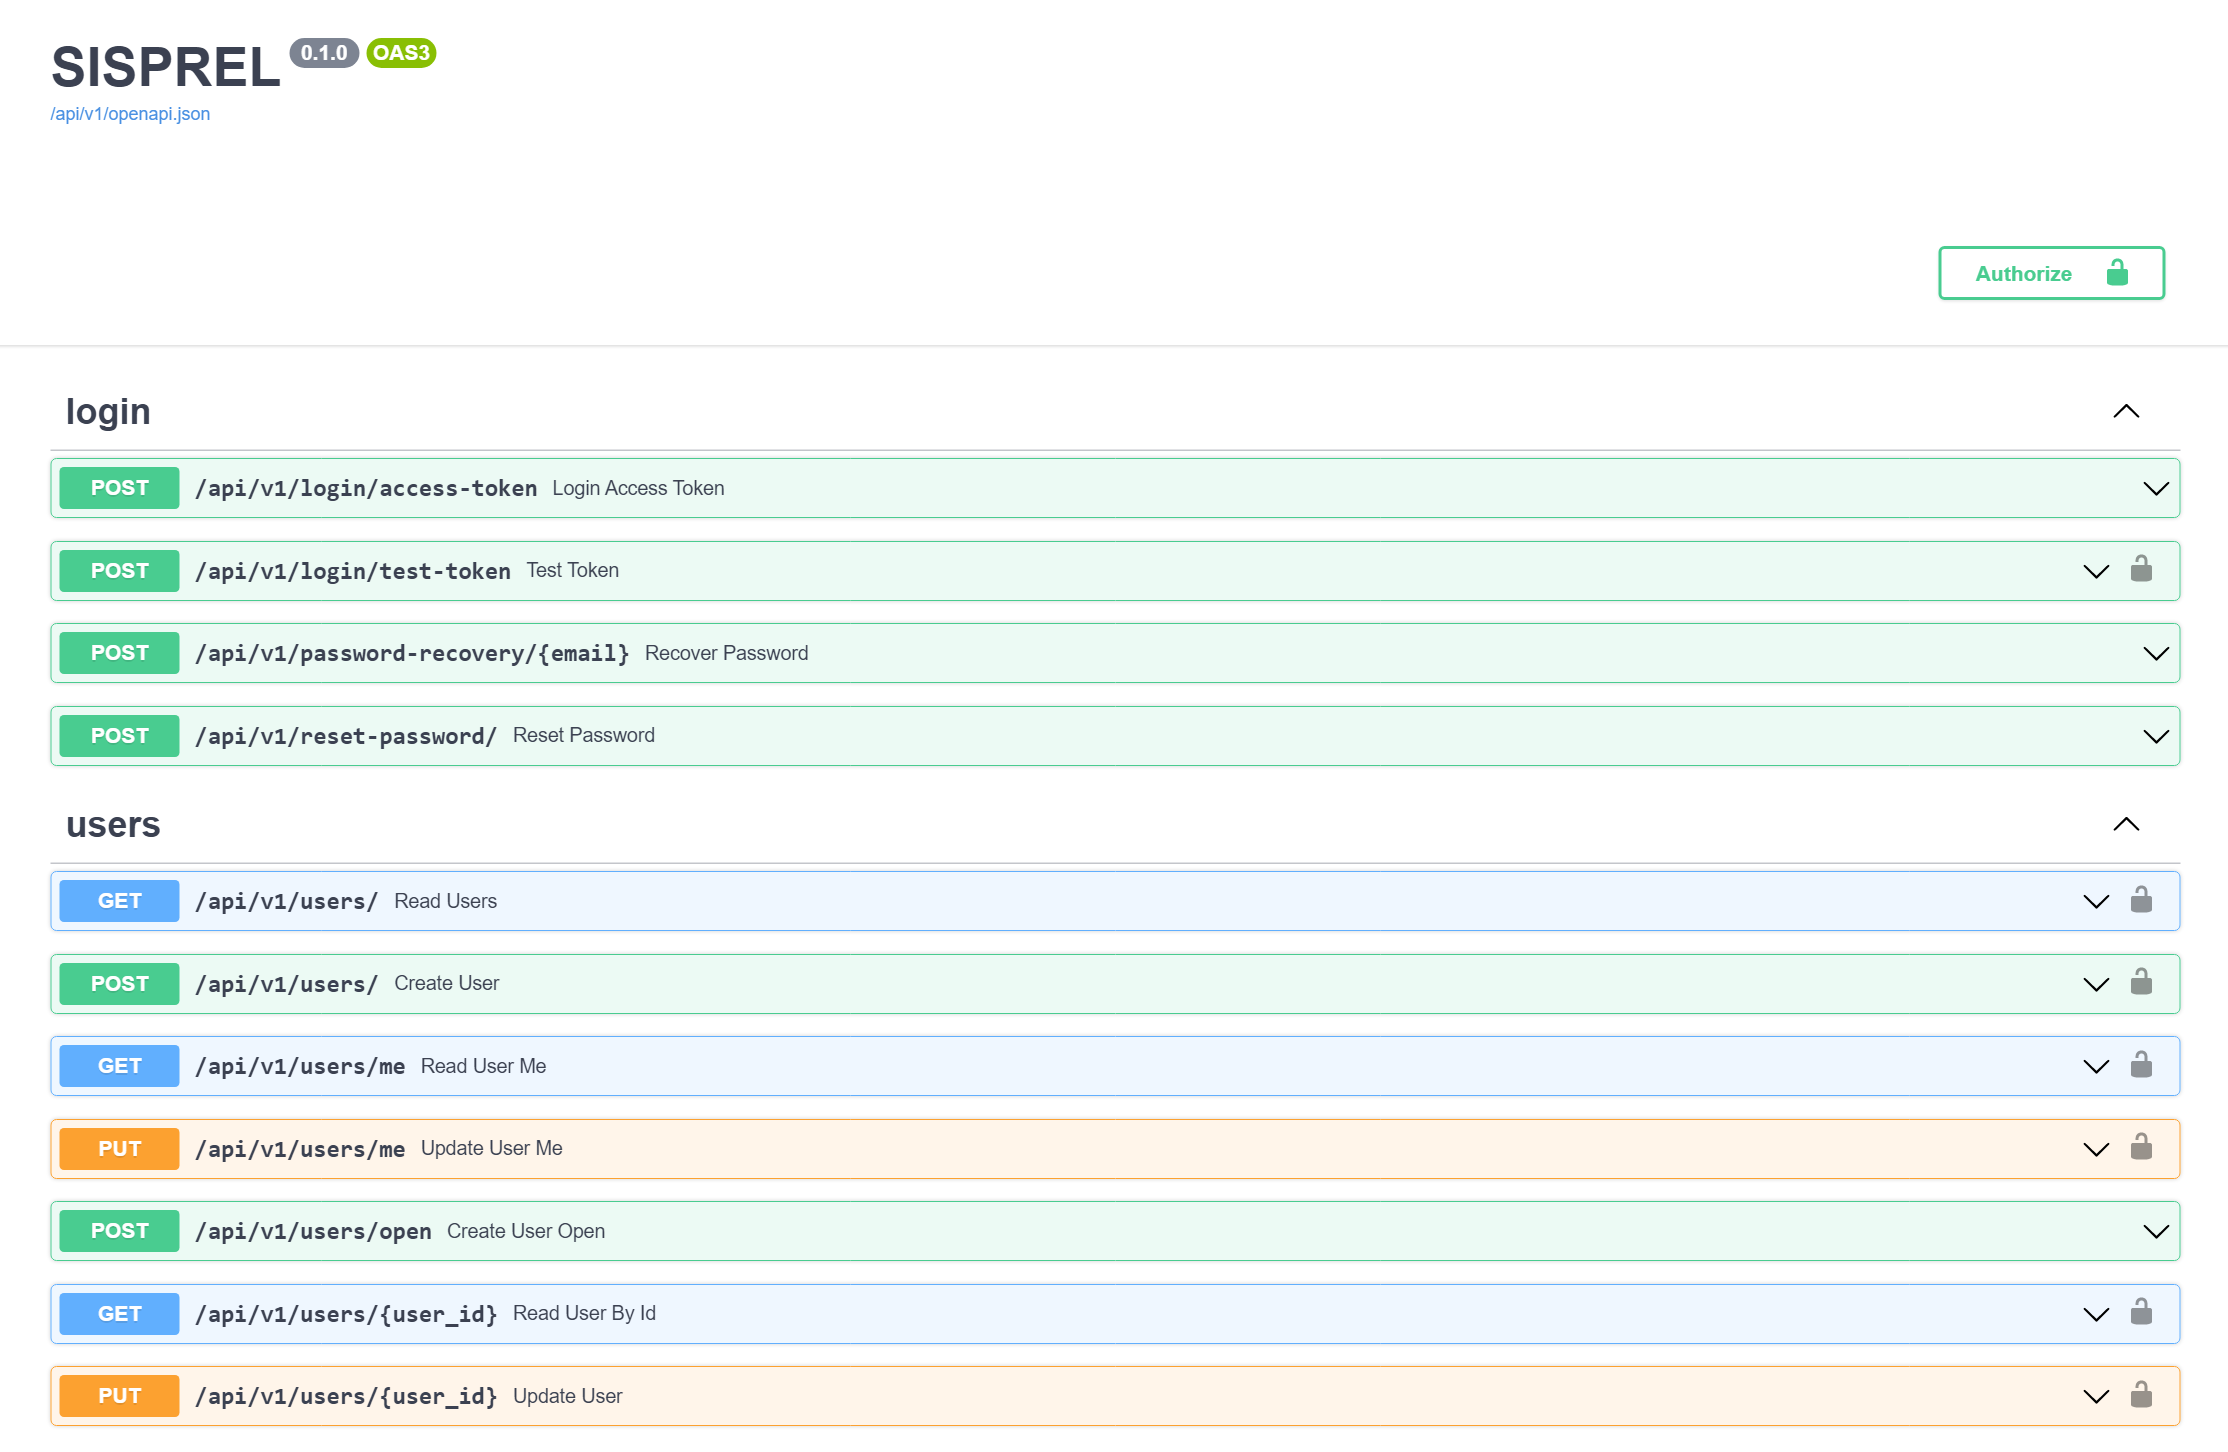
\includegraphics[scale=.20]{TT/img/implementacion/docs_1.png}
    \caption{Documentación 'docs' - Parte 1}
    \label{graphic:docs1}    
\end{figure}

Como se ha descrito anteriormente, esta versión de la documentación permite realizar pruebas, por lo tanto, para tener acceso a los endpoint que estan bloqueados, procedemos a iniciar sesión, en la imagen \ref{graphic:docs1} se puede observar un botón llamado Authorize, al darle clic nos mostrará un aviso como se puede apreciar en la imagen \ref{graphic:docs2} en donde nos pide algunos datos, los únicos que se van a requerir para acceder al sistema, ya sea con el uso de esta documentación o en cualquier aplicación que la consuma, es requerido ingresar el "username" que es el correo electrónico y la contraseña. Al ingresarlos y que sean correctos, nos sale otro aviso de que ha sido aprobada nuestra autorización  como se aprecia en la imagen \ref{graphic:docs3} y se nos otorga un token, el cual nos dará acceso a los endpoints del sistema y nos permite realizar las peticiones que estén disponibles.

\begin{figure}[!htb]
    \centering
    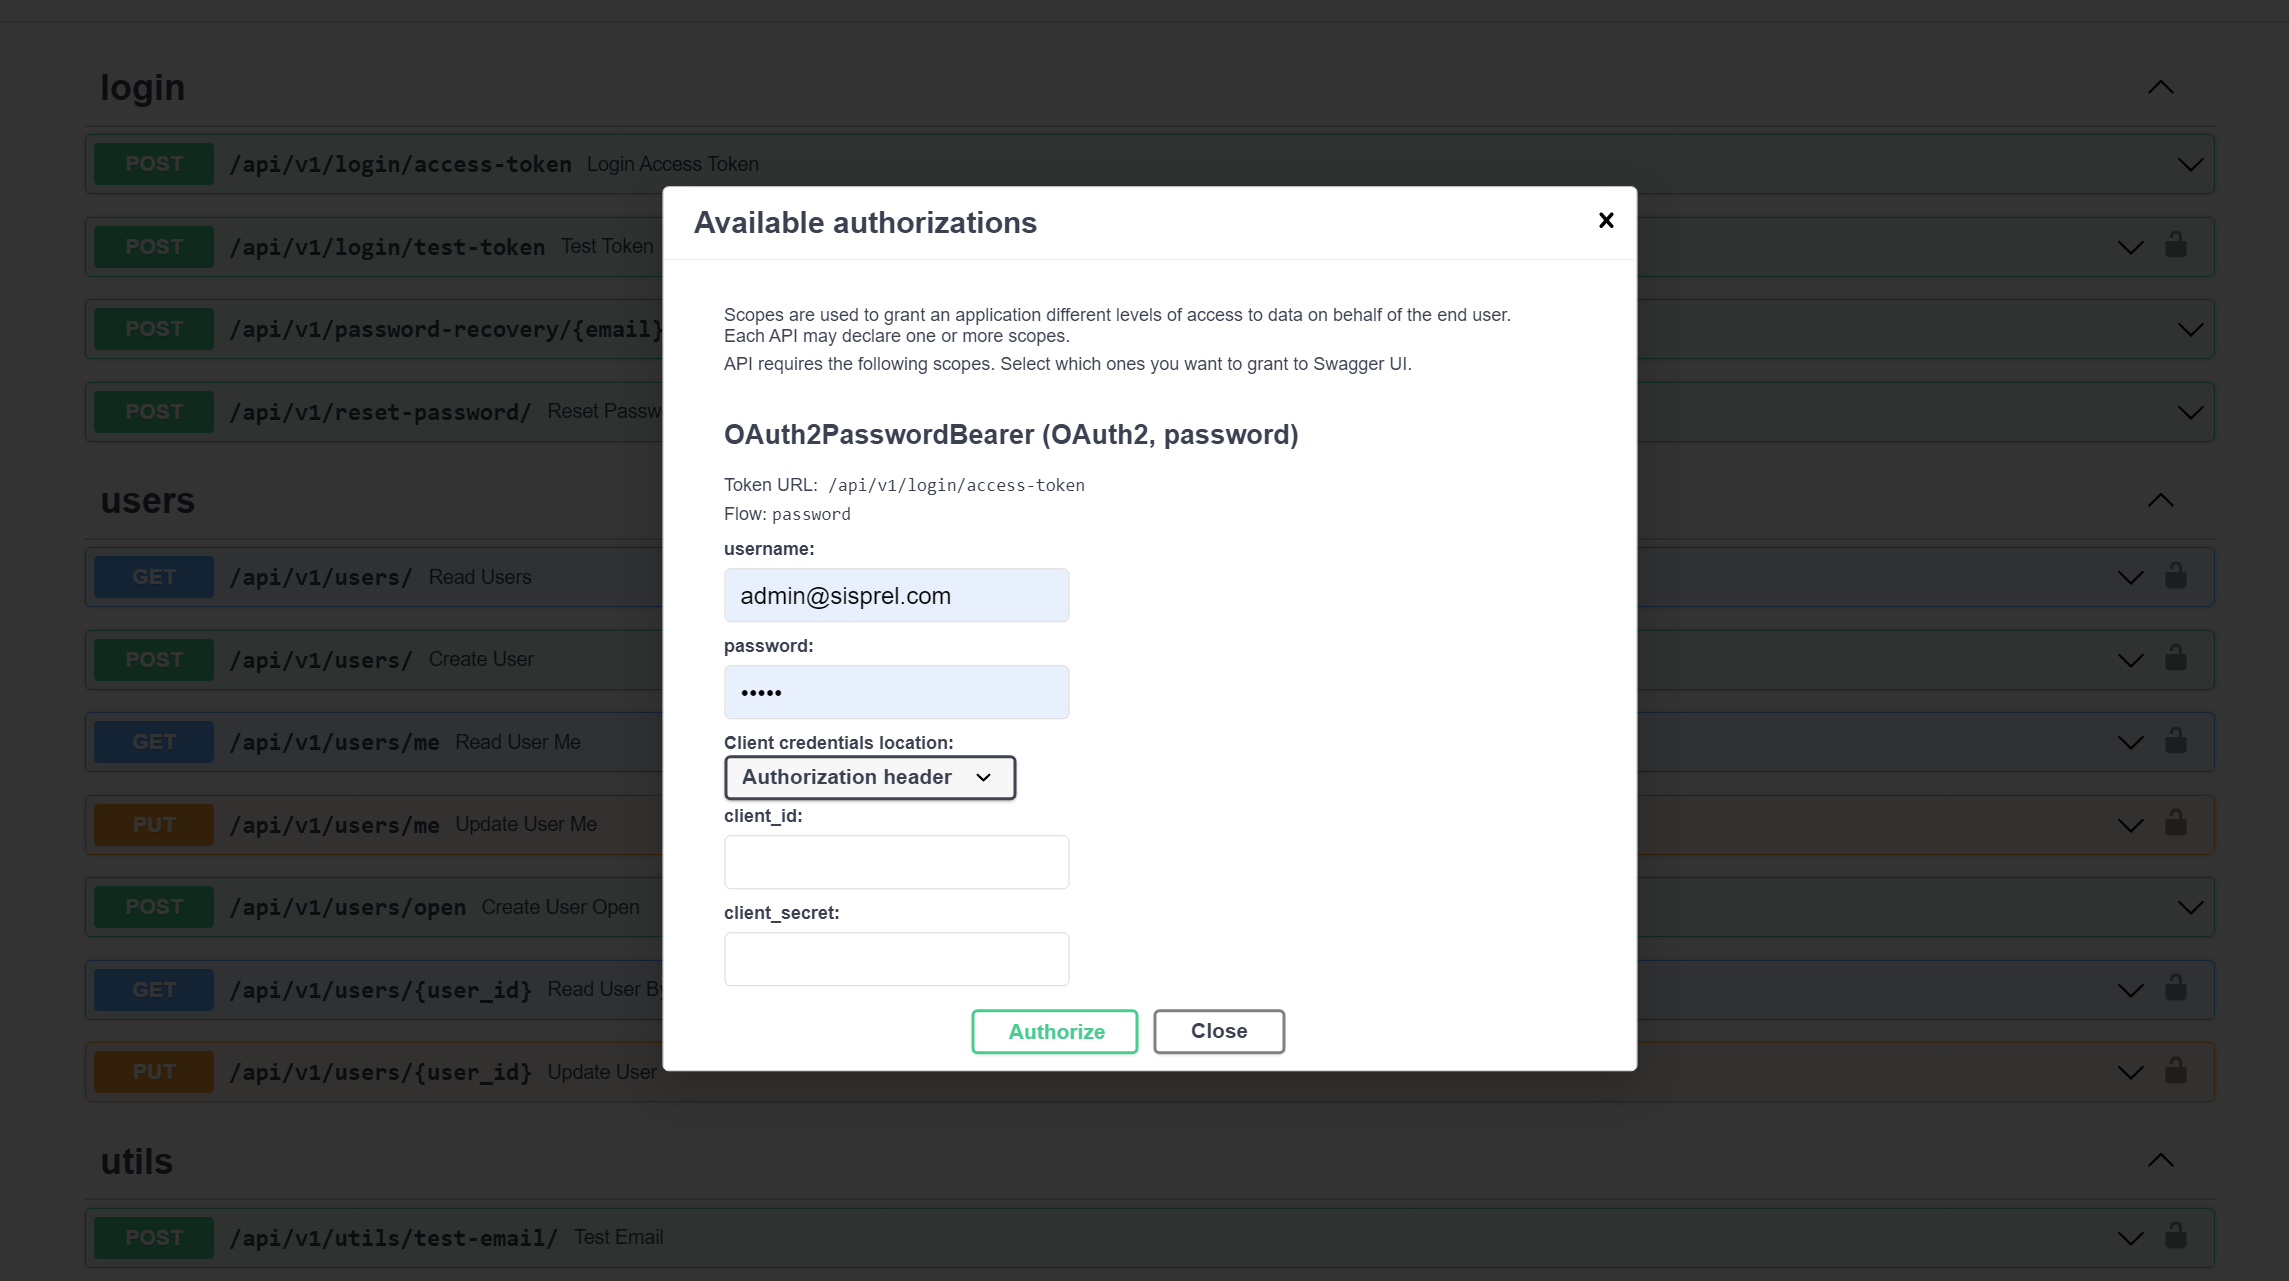
\includegraphics[scale=.20]{TT/img/implementacion/docs_2.png}
    \caption{Documentación 'docs' - Parte 2}
    \label{graphic:docs2}    
\end{figure}

\begin{figure}[!htb]
    \centering
    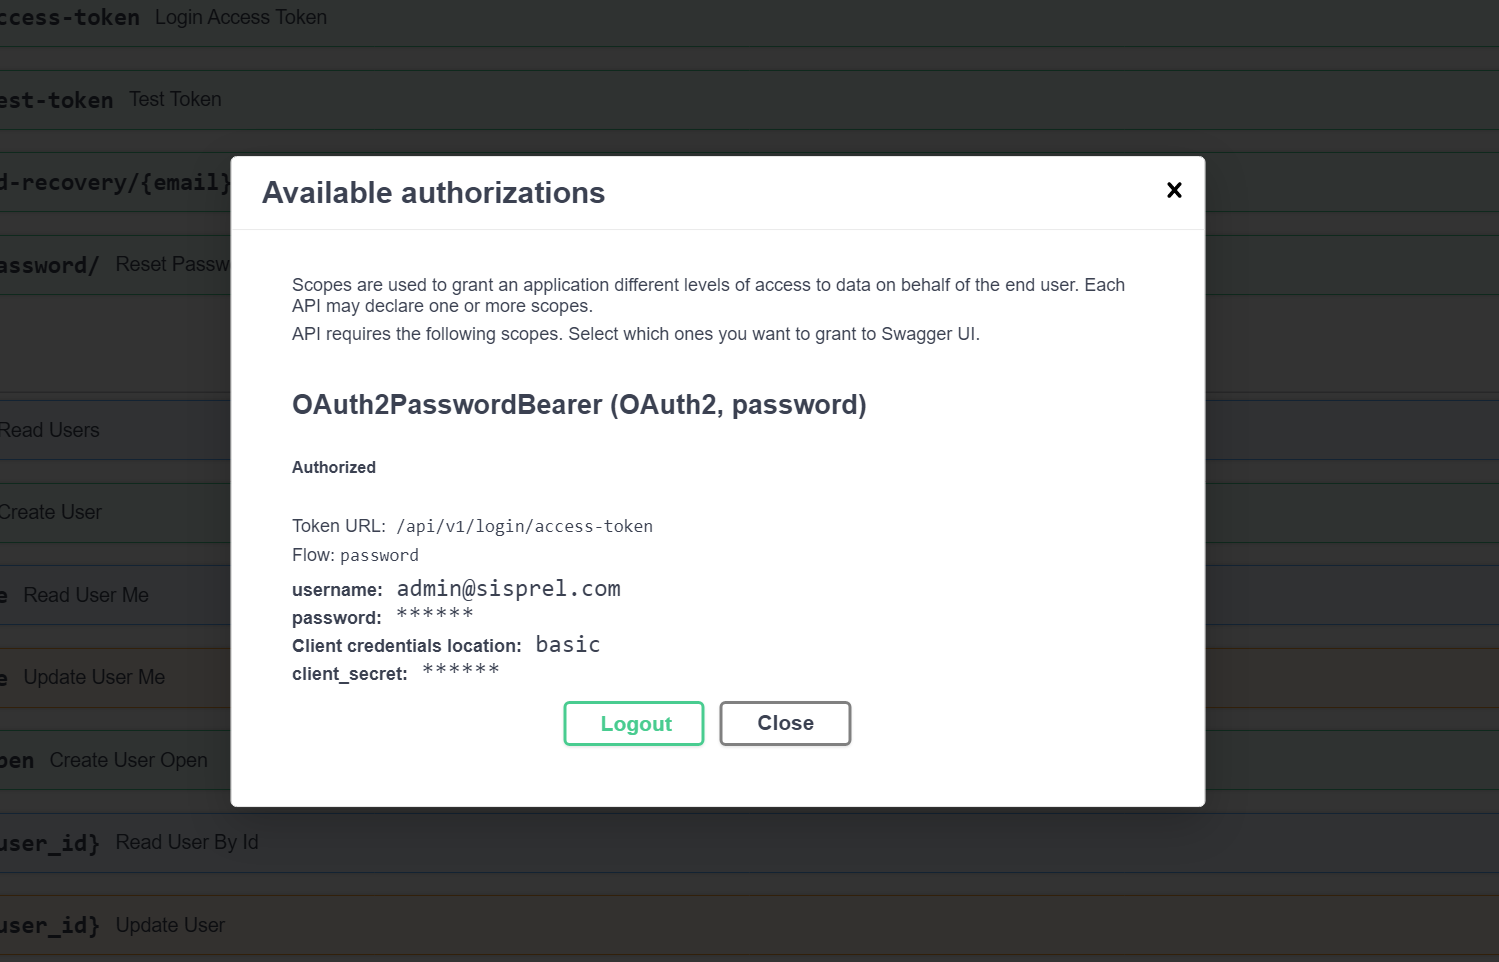
\includegraphics[scale=.30]{TT/img/implementacion/docs_3.png}
    \caption{Documentación 'docs' - Parte 3}
    \label{graphic:docs3}
\end{figure}

Teniendo el token de acceso, podemos realizar pruebas en los endpoints blindados, pero sin el, también podemos probar endpoints pero solo los que no están blindados. En la figura \ref{graphic:docs4} se muestra la interfaz del endpoint, al seleccionarlo nos muestra que datos hay que enviar y como va a devolver la respuesta la API, un código 200 significa que la petición ha sido cumplida y nos devuelve lo que hemos creado o pedido, un error 422 es un error de validación, ya sea porque se mandó algo mal o que no respeta el tipo de dato que se requiere y un error 402 es porque no tenemos autorización a ese recurso.

\begin{figure}[!htb]
    \centering
    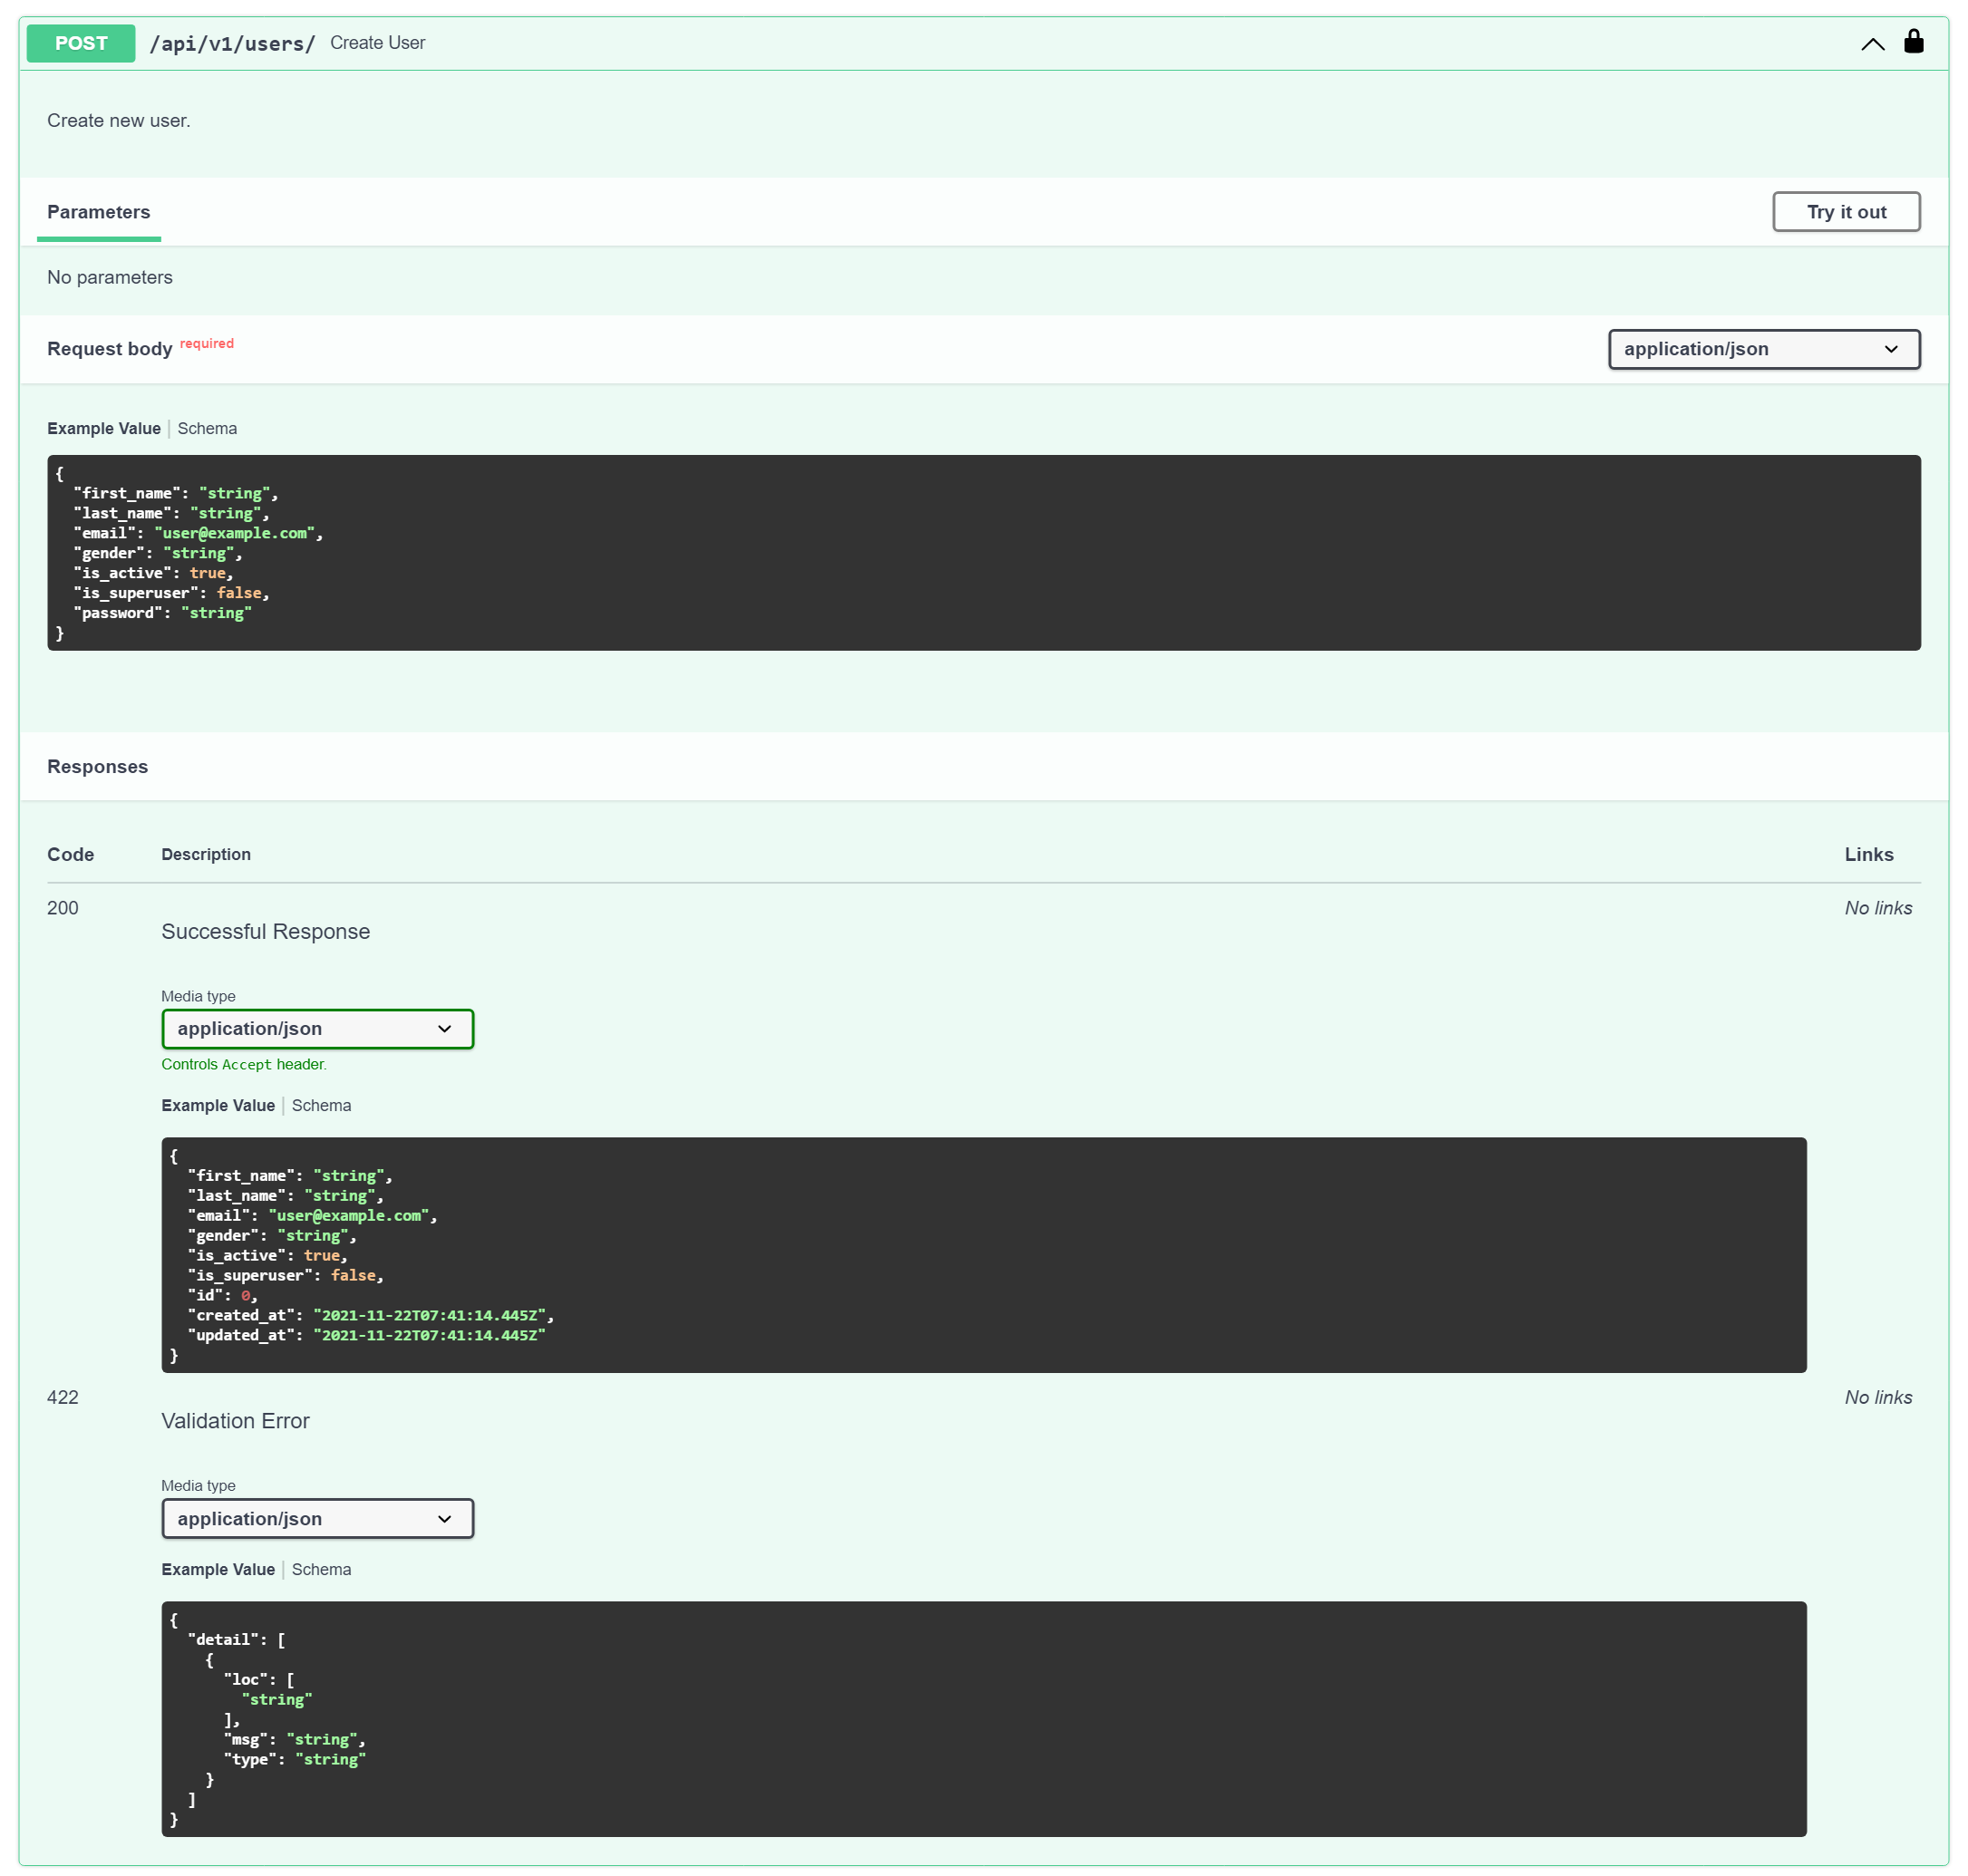
\includegraphics[scale=.20]{TT/img/implementacion/docs_4.png}
    \caption{Documentación 'docs' - Parte 4}
    \label{graphic:docs4}
\end{figure}

Como se mencionó en el parrafo anterior, se pueden realizar pruebas a la API desde esta página, lo que nos evita usar software de terceros para realizarlas tal como lo es por ejemplo Postman, para acceder a ello le damos clic al boton 'Try it out' nos habilitará una sección para mandar un JSON en el caso de realizar un POST a la API, un ID para la consulta o la eliminación de un objeto en la base de datos, en el caso de la imagen \ref{graphic:docs5} se presenta el caso para crear un usuario, por lo tanto se habilitarán los campos en formato JSON y el tipo de dato que este tiene que tener, se tiene que respetar el nombre del campo y se modifican los campos que se desea cambiar y  con ello, le damos clic al botón 'Execute' para ejecutar la petición y nos regresará el código y resultado correspondiente.

\begin{figure}[!htb]
    \centering
    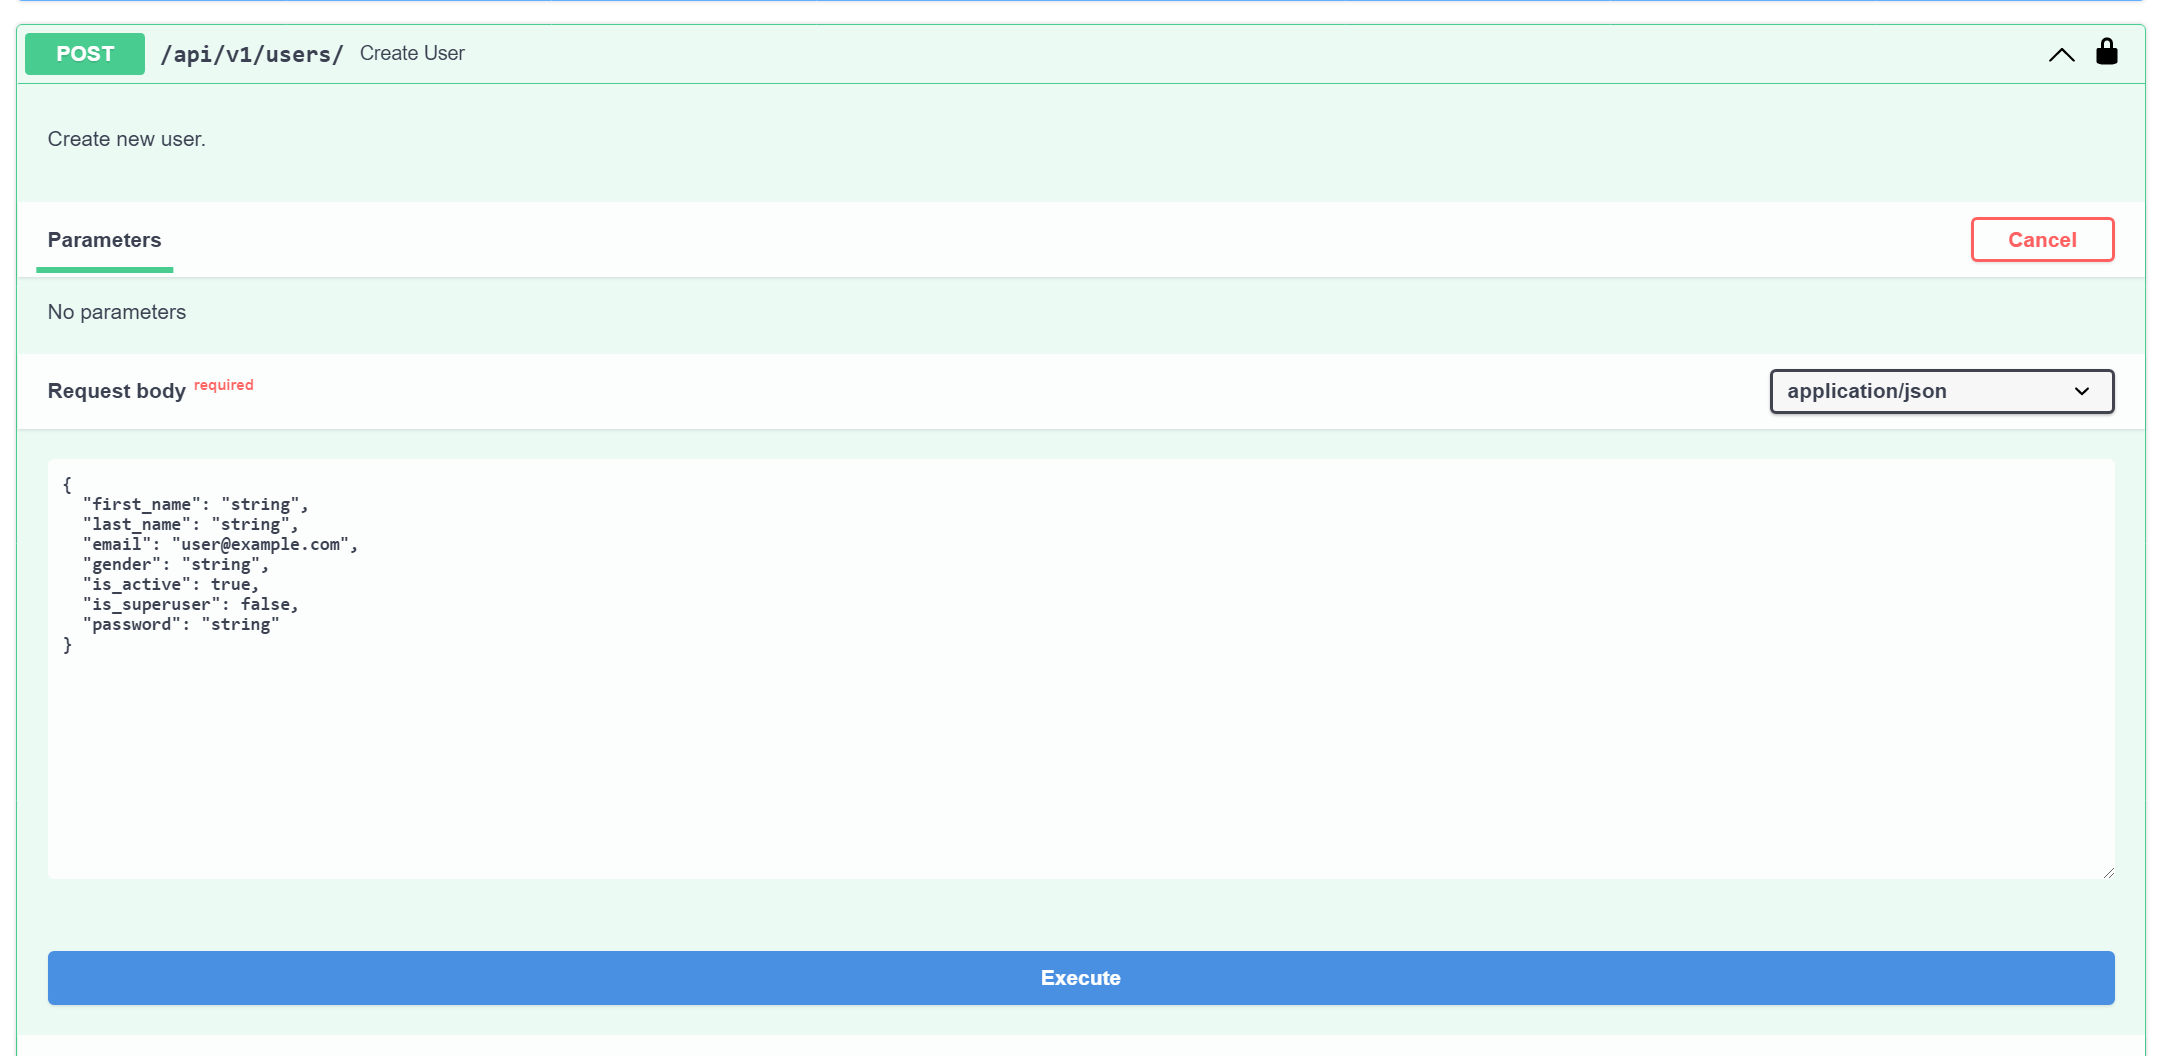
\includegraphics[scale=.20]{TT/img/implementacion/docs_5.png}
    \caption{Documentación 'docs' - Parte 5}
    \label{graphic:docs5}
\end{figure}

Por último, esta versión de la documentación nos genera la lista de los esquemas usados por la API mostrados en la imagen \ref{graphic:docs6}, estos contienen el nombre del esquema y que es lo que pueden recibir o devuelven en formato JSON de acuerdo al tipo de petición que se realice.
\begin{figure}[!htb]
    \centering
    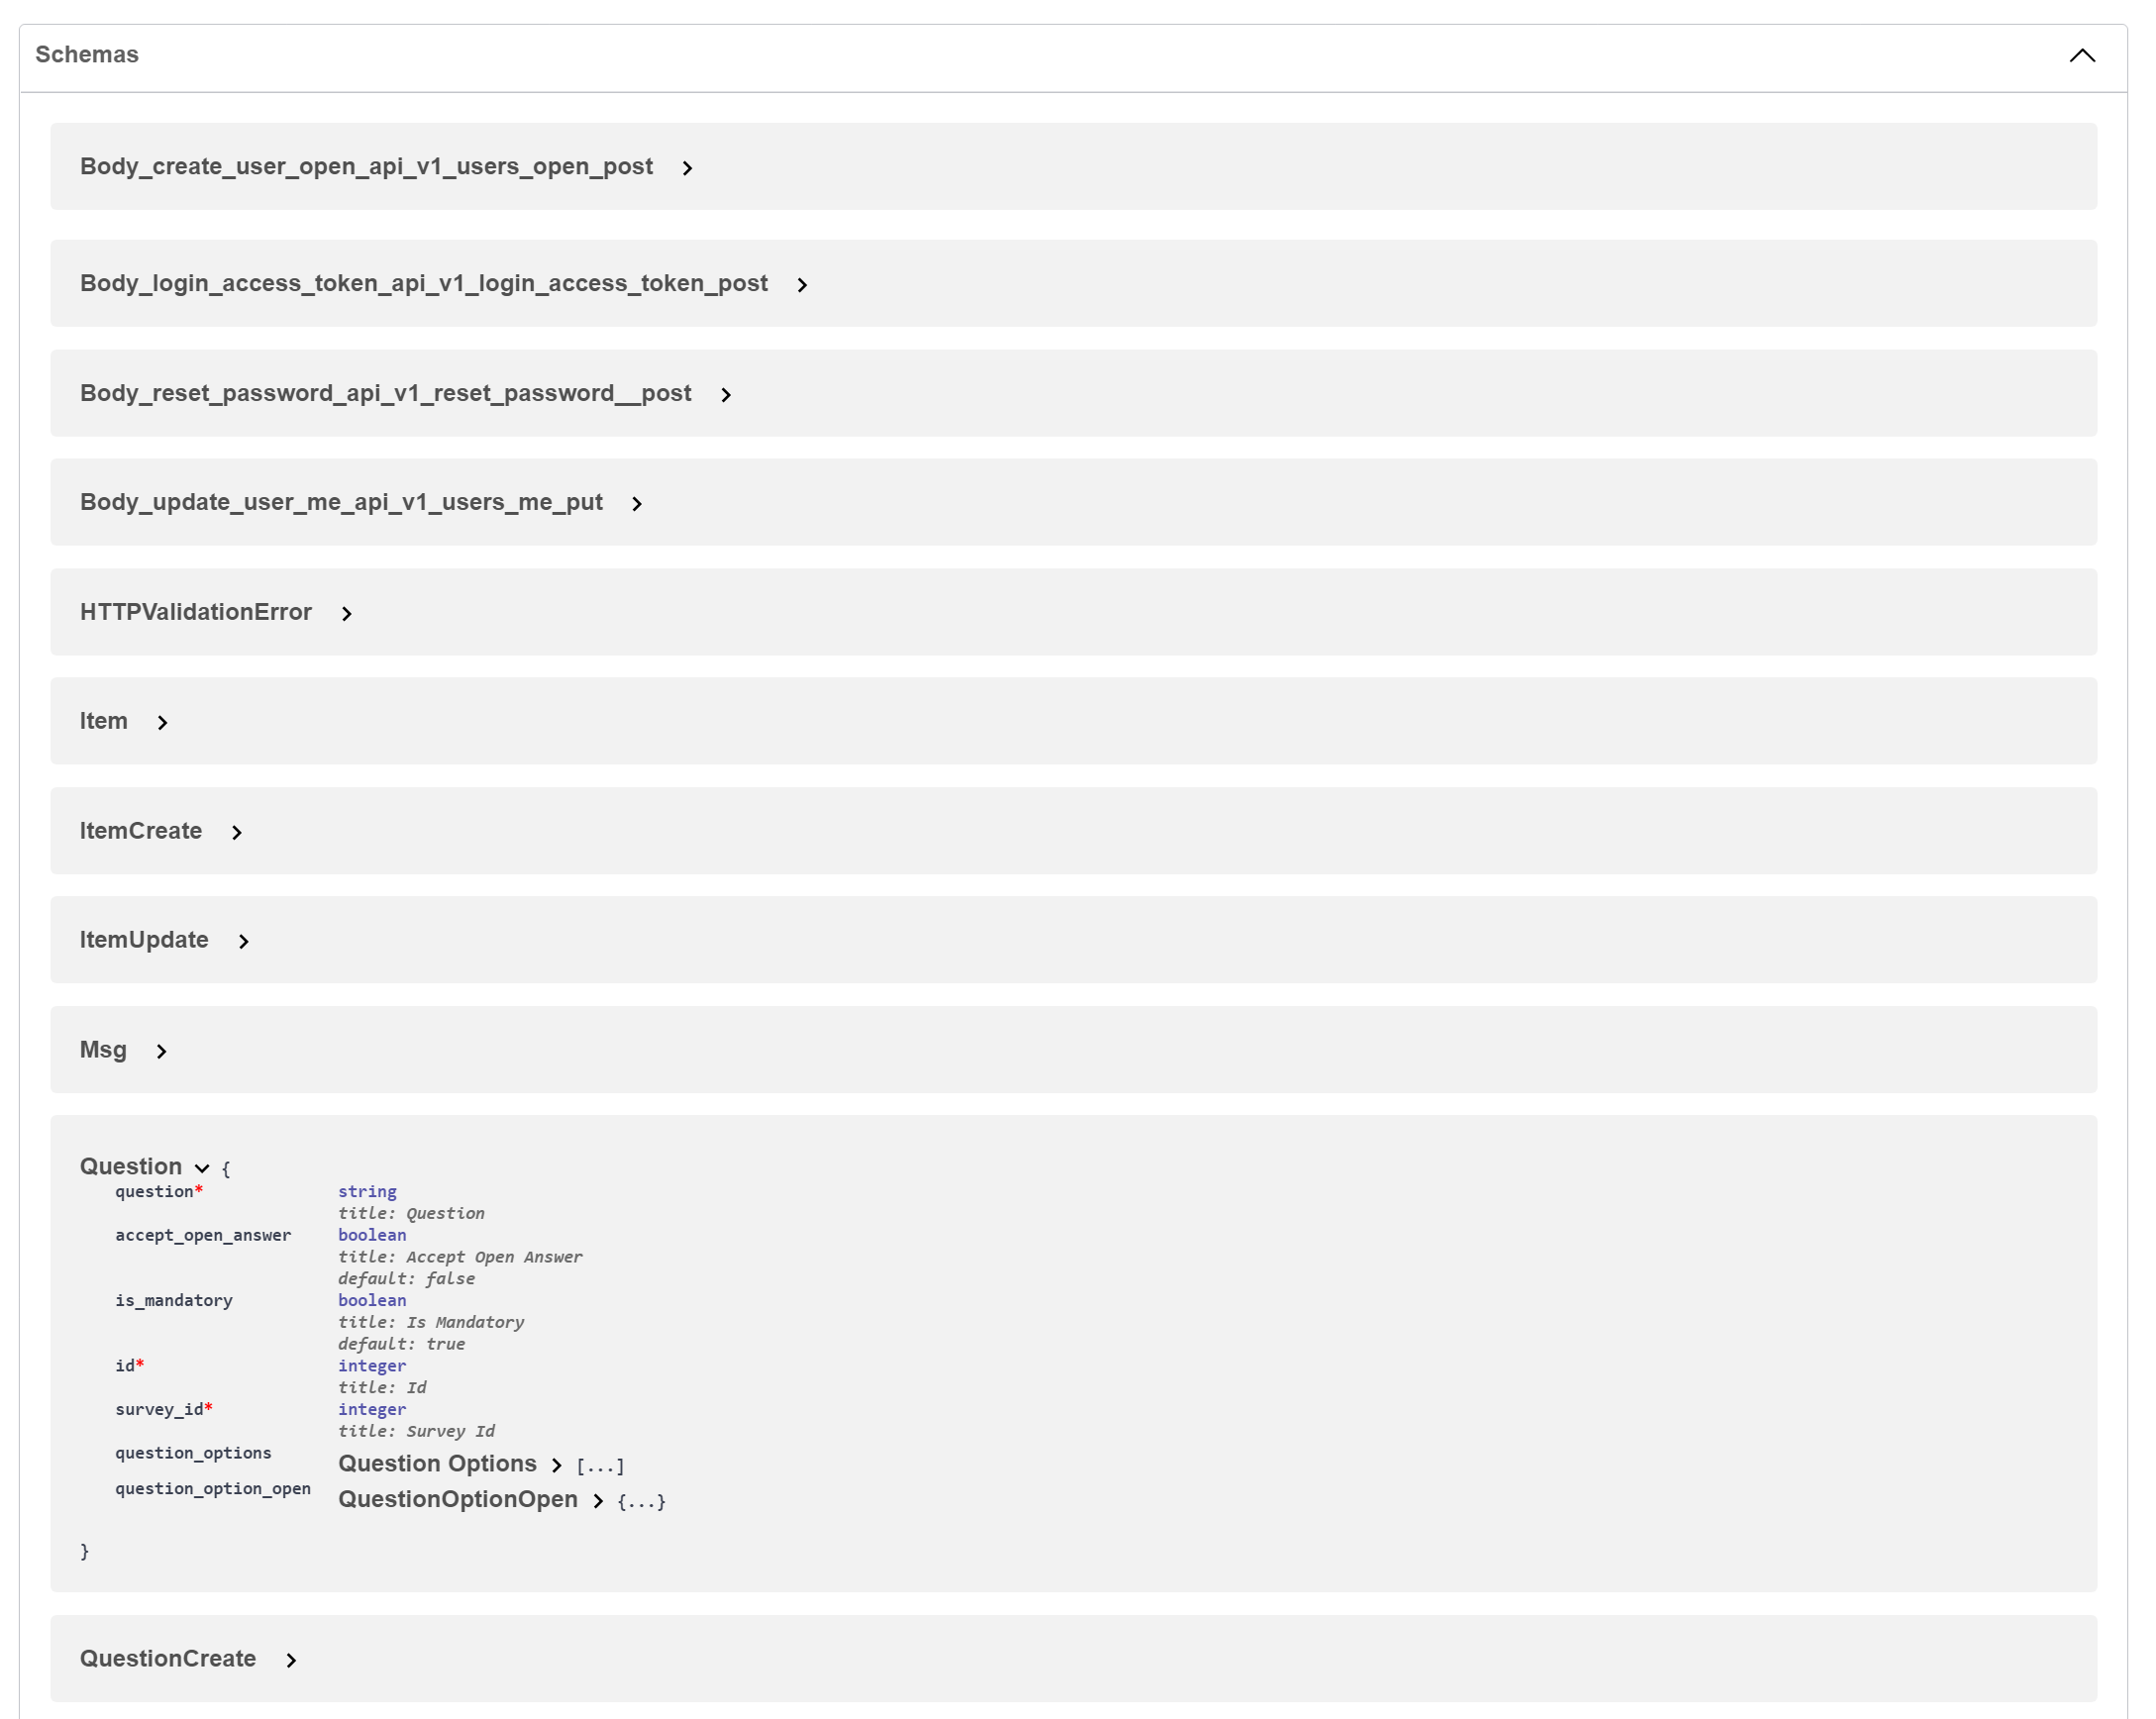
\includegraphics[scale=.20]{TT/img/implementacion/docs_6.png}
    \caption{Documentación 'docs' - Parte 6}
    \label{graphic:docs6}
\end{figure}

\subsubsection{Documentación de FastApi - 'redoc'}
Esta versión esta enfocada en la explicación sobre cada endpoint y los esquemas, en la figura \ref{graphic:redoc1} se puede apreciar la diferencia con la sección anterior. La interfaz de usuario se enfoca mas en informar al usuario la estructura de los endpoint y que datos requiere la API para realizar las peticiones que el usuario desea hacer.

\begin{figure}[!htb]
    \centering
    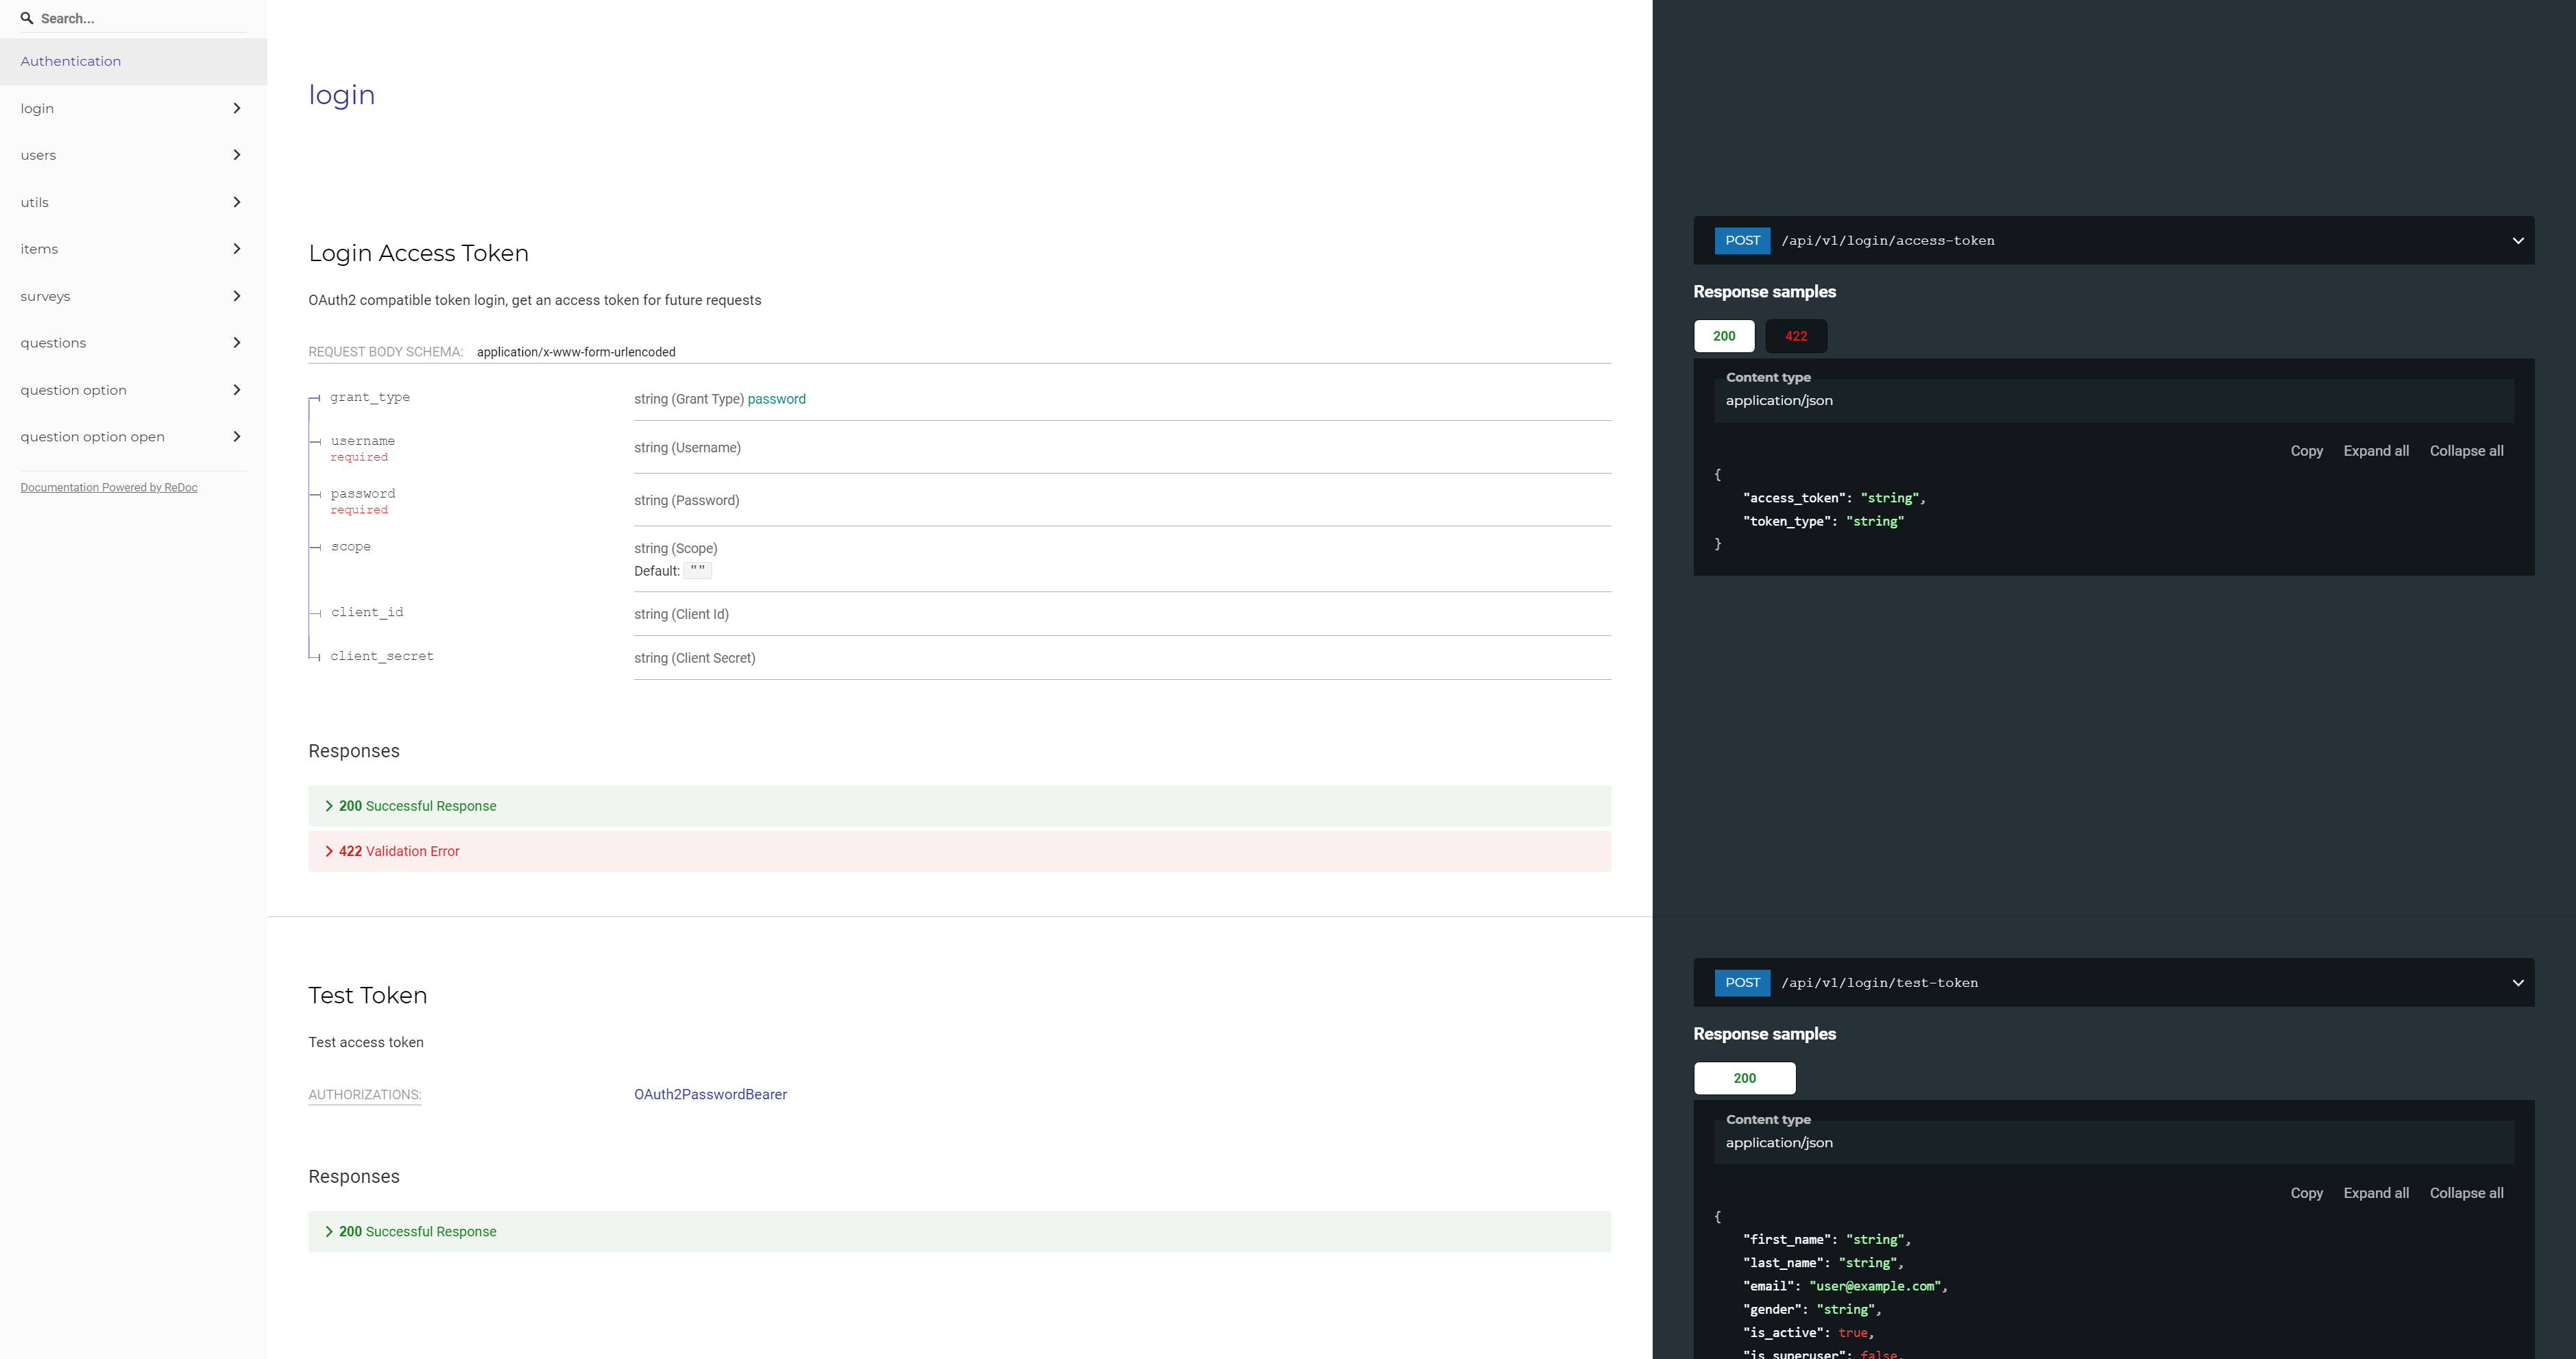
\includegraphics[scale=.25]{TT/img/implementacion/redoc_1.png}
    \caption{Documentación 'redoc' - Parte 1}
    \label{graphic:redoc1}
\end{figure}

En la imagen \ref{graphic:redoc2} se muestra la documentación del endpoint para crear usuario, del lado izquierdo estan listados los endpoint y al darle clic al que se desee, en este caso el endpoint de \textit{users} muestra las peticiones que se pueden hacer y el nombre de estas; en la parte central viene el nombre de la petición, describe el tipo de autorización que se requiere para poder usar el endpoint, describe como es el cuerpo el esquema de la petición los nombres de los campos y el tipo de dato que permite y al final viene detallada las respuestas.
\begin{figure}[!htb]
    \centering
    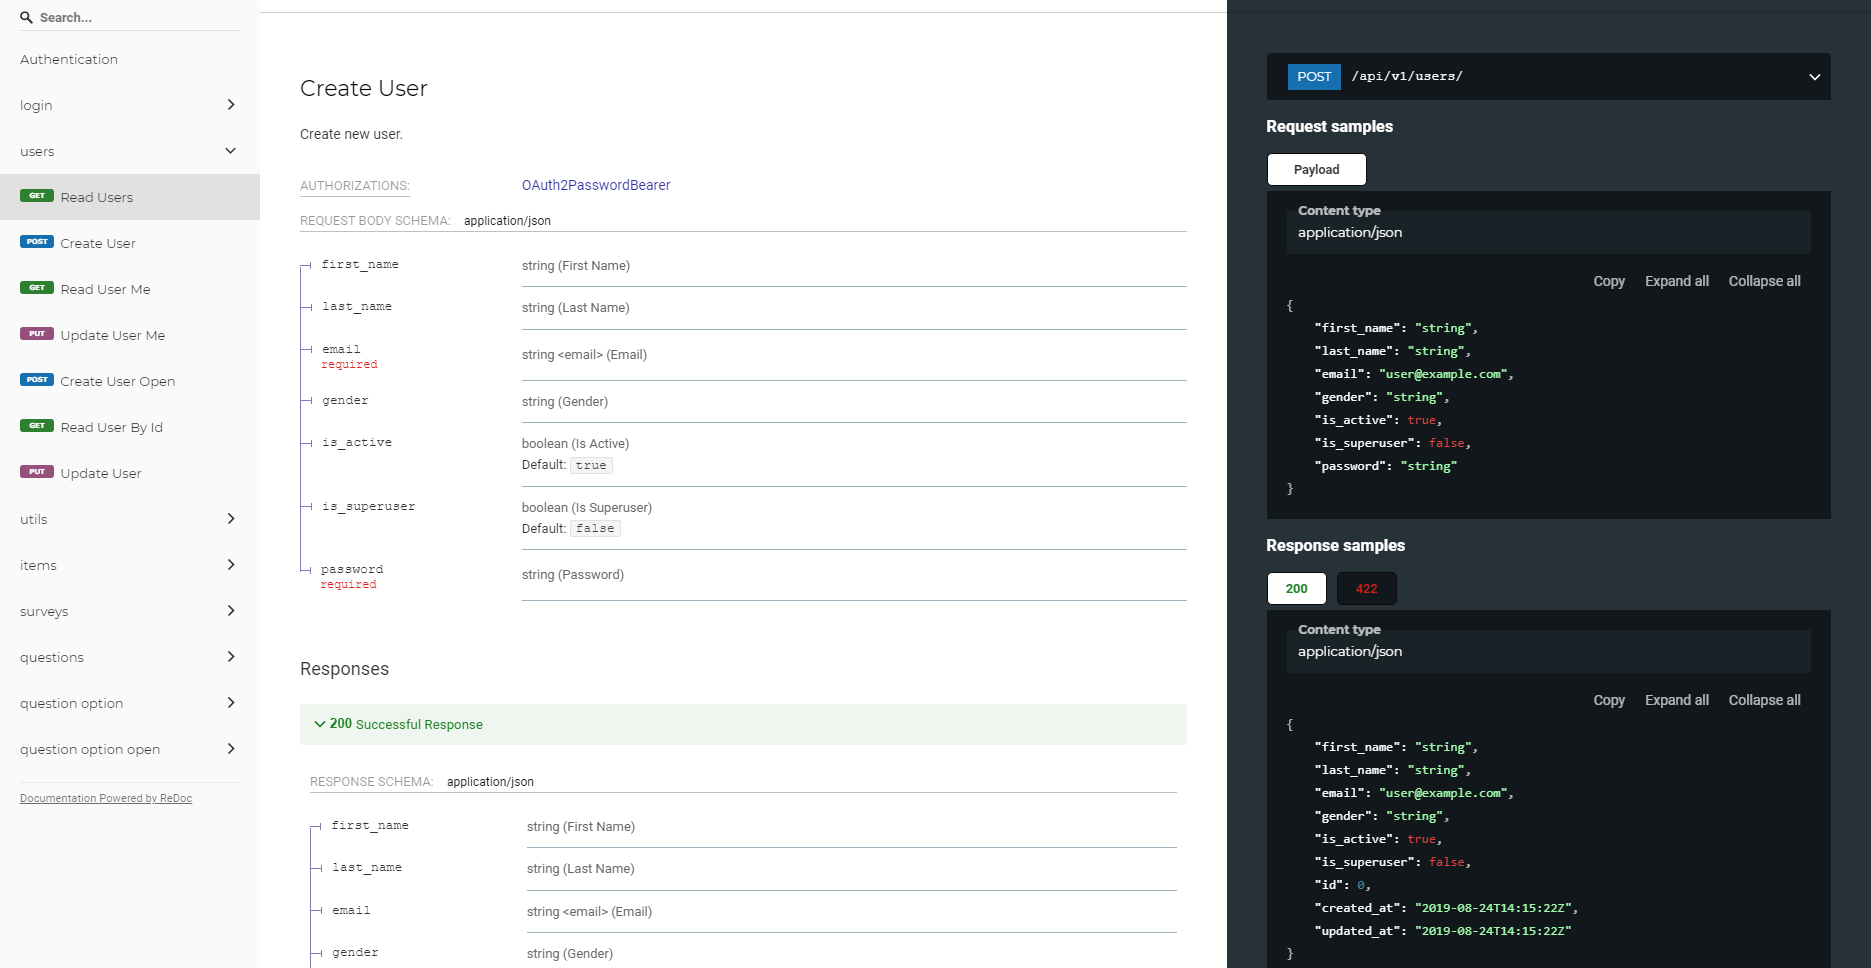
\includegraphics[scale=.25]{TT/img/implementacion/redoc_2.png}
    \caption{Documentación 'redoc' - Parte 2}
    \label{graphic:redoc2}
\end{figure}

Por último, en la imagen \ref{graphic:redoc3} y \ref{graphic:redoc4} se ve con mas detalle lo que se mostraba en las imágenes \ref{graphic:redoc1} y \ref{graphic:redoc2} del lado izquierdo, en esta sección detalla con mas precisión el endpoint, en la parte de arriba de las imágenes se muestra el tipo de petición y la URL de este mismo y al hacer clic de en el URL, nos desplegará el URL con el dominio en el que este configurado para su acceso mostrándose en la imagen \ref{graphic:redoc4}. En la parte central se muestra como se envían los datos, en todos los casos son 'aplication/json' junto con los campos y un ejemplo de como se deben de llenar para realizar la petición. Al final,

\begin{figure}[!htb]
    \centering
    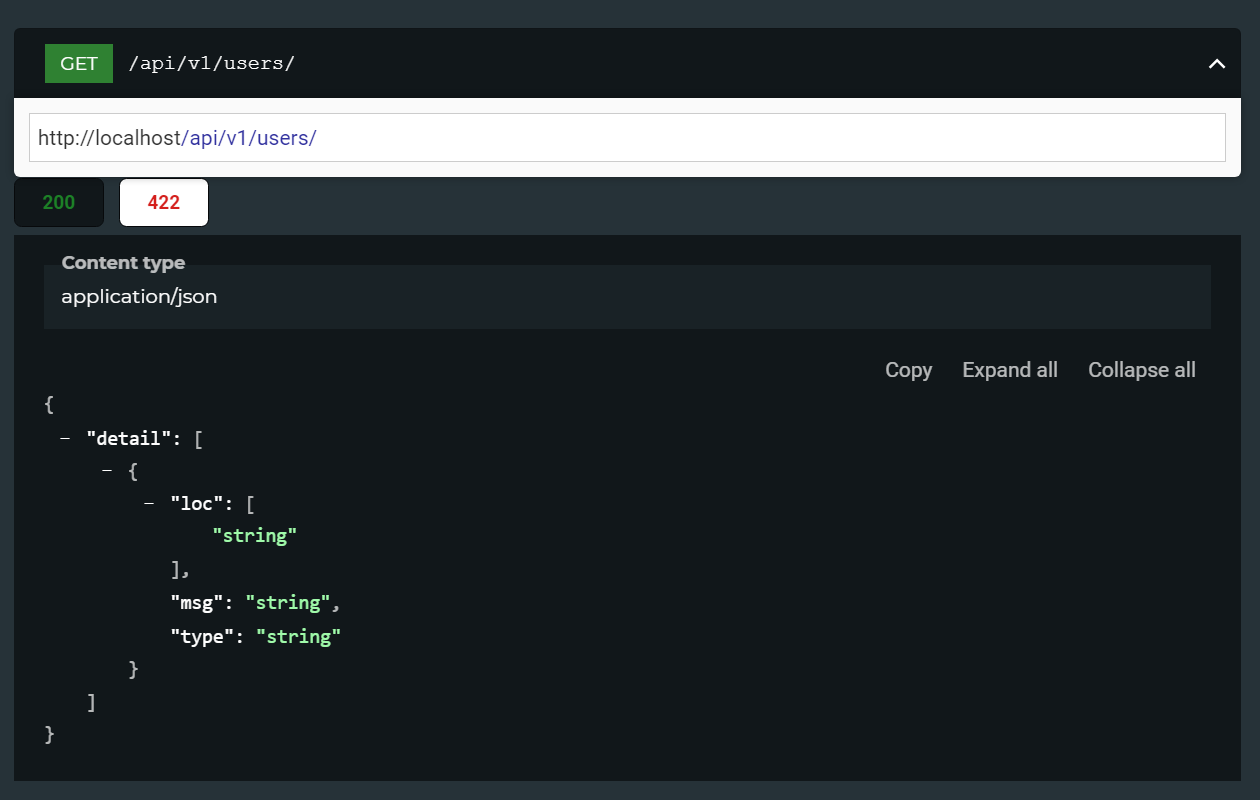
\includegraphics[scale=.40]{TT/img/implementacion/redoc_3.png}
    \caption{Documentación 'redoc' - Parte 3}
    \label{graphic:redoc3}
\end{figure}

\begin{figure}[!htb]
    \centering
    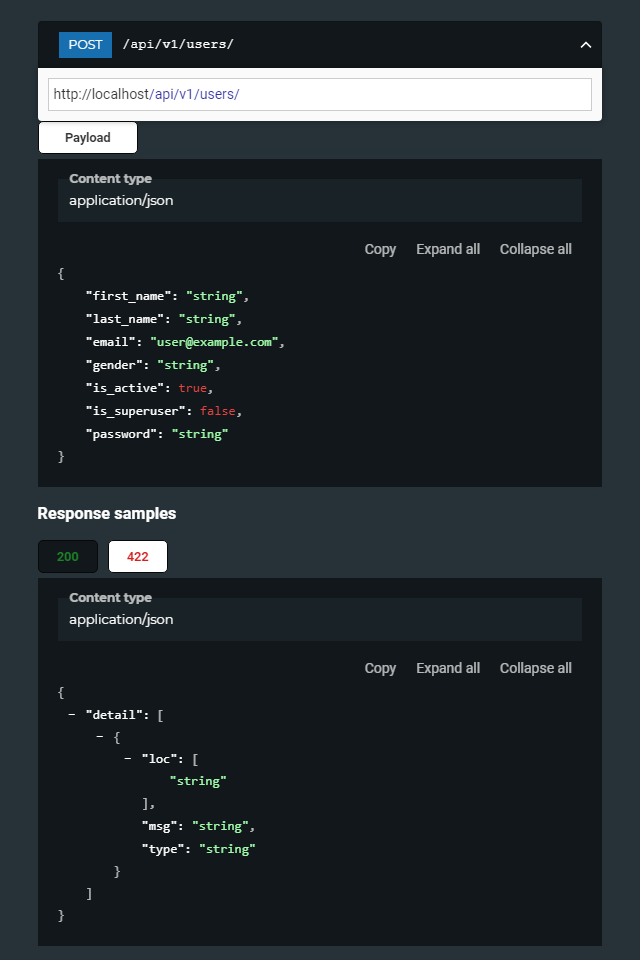
\includegraphics[scale=.40]{TT/img/implementacion/redoc_4.png}
    \caption{Documentación 'redoc' - Parte 4}
    \label{graphic:redoc4}
\end{figure}

\subsection{VueJS}
Para consumir la API usando una interfaz de usuario, se ha elegido usar el framework VueJS de JavaScript por su sencillez.
\subsubsection{Estructura del Frontend}
\subsubsection{Typescript}
\subsubsection{Interfaz de usuario}

